\documentclass{amsart}
\usepackage{amsmath}
\usepackage{bbm} % allows for \mathbb{}-like numbers
\usepackage{amssymb}
\usepackage{proof}
\usepackage{cancel}
\usepackage[usenames,dvipsnames]{color}
\usepackage{graphics}
\usepackage{verbatim}
\usepackage{tikz}

\usetikzlibrary{arrows}

\usepackage{caption}
\usepackage[all]{xy} 

\theoremstyle{definition}

\newtheorem{thm}{Theorem}[section]
\newtheorem{cor}[thm]{Corollary}
\newtheorem{lem}[thm]{Lemma}
\newtheorem{conjecture}[thm]{Conjecture}
\newtheorem{definition}[thm]{Definition}
\newtheorem{proposition}[thm]{Proposition}
\newtheorem{example}[thm]{Example}

\newcommand{\truls}[1]{\textbf{\textcolor{magenta}{(T: #1)}}}
\newcommand{\sjur}[1]{\textbf{\textcolor{blue}{(S: #1)}}}
\newcommand{\piotr}[1]{\textbf{\textcolor{OliveGreen}{(P: #1)}}}
\newcommand{\erik}[1]{\textbf{\textcolor{Peach}{(E: #1)}}}
\newcommand{\todo}[1]{\textcolor{Red}{\footnote{TODO: #1}}}

\newcommand{\nn}{\mathbb N} % the natural numbers
\newcommand{\rr}{\mathbb R} % the real numbers
\newcommand{\ca}{\mathcal A} % arbitrary algebra A (\ca = caligraphic A)
\newcommand{\cb}{\mathcal B} % arbitrary algebra B (\cb = caligraphic B)

% how about some consistent conventions?
% T: okay. here you go.
\newcommand{\cat}[1]{\mathsf{#1}} % Specific category, e.g., Set
\newcommand{\acat}[1]{\mathbb{#1}} % Arbitrary category, e.g., C

\begin{document}

\section{Background and history}
\begin{description}
\item[Abstract systems] (Emmy Noether)

\begin{quote}
Amalie Emmy Noether (German: [ˈnøːtɐ]; 23 March 1882 – 14 April 1935), sometimes referred to as Emily[1] or Emmy, was an influential German mathematician known for her groundbreaking contributions to abstract algebra and theoretical physics. Described by Pavel Alexandrov, Albert Einstein, Jean Dieudonné, Hermann Weyl, Norbert Wiener and others as the most important woman in the history of mathematics,[2][3] she revolutionized the theories of rings, fields, and algebras. In physics, Noether's theorem explains the fundamental connection between symmetry and conservation laws.[4] (wikipedia)\end{quote}

\item[Universal Algebra] Garrett Birkhoff
\begin{quote}
Garrett Birkhoff (January 19, 1911 – November 22, 1996) was an American mathematician. He is best known for his work in lattice theory. (wikipedia)
\end{quote}

\begin{quote}The following paper is a study of abstract algebras qua abstract algebras. As no vocabulary suitable for this purpose is current, I have been forced to use a number of new terms, and extend the meaning of some accepted ones. (abstract, ``On the structure of Abstract Algebra'' 1935)
\end{quote}
\end{description}

\section{Behaviour and processes}

\piotr{I'll write this maybe tomorrow\ldots}

\section{Mathematical Preliminaries}

\begin{definition}\textbf{(Stream)} A \textit{stream} $(S, \leq)$ over alphabet $A$ is a subset of lists over $A$, $S \subseteq A^\ast$ together with an ordering $\leq$ such that
\begin{itemize}
\item $(S, \leq)$ is linearly ordered, and
\item $(S, \leq)$ is prefix closed.
\end{itemize}
\end{definition}

\begin{example} Here is an example of a~stream: $01010101010101\ldots$, where $S = \{0,01,010,0101,\ldots\}$ and the order is defined as $0 \leq 01\leq 010\leq 0101\leq\ldots$
\end{example}

\begin{definition}\textbf{(Infinite Tree)} An \textit{infinite tree} is like a stream, but not linearly ordered.
\end{definition}

\begin{definition}\textbf{(Algebra)} An \textit{algebra} is a tuple $(C, op_1, \dots, op_n)$ where
\begin{itemize}
\item $C$ is a non-empty set called the \textit{carrier set}, and
\item for each $1 \leq i \leq n$, $op_i : C^x \to C$, where $x$ is the arity, i.e.\ $x = ar(op_{i})$. 
\end{itemize}
\end{definition}

\begin{definition}\textbf{(Signature)} A \textit{signature} is a pair $\Sigma = (OP, ar)$ where
\begin{itemize}
\item $OP$ is a set of operation names, and
\item $ar : OP \to \mathbb N$ is the arity map.
\end{itemize}
\end{definition}

\begin{example} Here are some algebras.
  \begin{enumerate}
  \item $\mathcal N_1$ is an algebra with carrier set $\mathbb N$ and a single operation $s : \nn \to \nn$.
  \item $\mathcal N_2$ is an algebra with carrier set $\nn$ and two operations: $s : \nn \to \nn$ and $\_+\_ : \nn \times \nn \to \nn$.
  \item $\mathcal R_\ast$ is an algebra where the carrier set is the set of positive real numbers $\mathbb R_+$ and the three operations are the constant $1 : \rr_+^0 \to \rr_+$ (or $1 : \mathbf 1 \to \rr_+$), the unary map $\frac 1 \_ : \rr_+ \to \rr_+$, and the binary operation $\_*\_ : \rr_+^2 \to \rr_+$.
  \item $\mathcal L$ is a \textit{two-sorted} algebra (of lists) where the carriers are $\nn$ and $\nn^\ast$, the operations are
    \begin{itemize}
    \item a constant (empty list) $[\ ] : \mathbf 1 \to \nn^\ast$,
    \item binary (building) $\_ :\_ : \nn \times \nn^\ast \to \nn^\ast$, and
    \item binary (concatination) $\_ ++ \_ : \nn^\ast \times \nn^\ast \to \nn^\ast$.
    \end{itemize}
  \item $\wp$ is a two-sorted algebra where the carrier sets are $\nn$ and $\wp \nn$, with operations
    \begin{itemize}
    \item constant $\emptyset : \mathbf 1 \to \wp \nn$,
    \item binary $\{\_\}\cup\_ : \nn \times \wp \nn \to \wp \nn$, and
    \item binary $\_ \cup \_ : \wp\nn \times \wp \nn \to \wp \nn$.
    \end{itemize}
  \end{enumerate}

  Here is a signature.
  \begin{enumerate}
    \item $\Sigma_1 = (OP_1, ar_1)$ where $OP_1 = \{c, u\}$, $ar_1(c) = 0$ and $ar_1(u) = 1$. 

      (The signature of a simple algebra with one constant and one unary operation.)
  \end{enumerate}
\end{example}

\begin{definition}\textbf{(Subalgebra)} An $\Sigma$-algebra $\ca$ is a subalgebra of $\Sigma$-algebra $\cb$ if
\begin{itemize}
\item $A \subseteq B$, and
\item $op^\ca = op^\cb \downarrow A^{ar(op)}$ for each $op \in OP$.
\end{itemize}
\end{definition}

If $\ca$ is a subalgebra of $\cb$, $A$ contains all constants and $A$ is closed under the operations in $\cb$.

\begin{definition}\textbf{(Homomorphism)} $f : \ca \to \cb$ is a \textit{$\Sigma$-homomorphism} from $\ca$ to $\cb$ if
\begin{itemize}
\item $f : A \to B$, and 
\item for all $op \in OP$ and all $(a_1, \dots, a_n) \in A^{ar(op)}$
$$f(op^\ca(a_1, \dots, a_n)) = op^\cb(f(a_1), \dots, f(a_n)).$$
\end{itemize}
or, more diagramatically, the following diagram commutes

\begin{center}
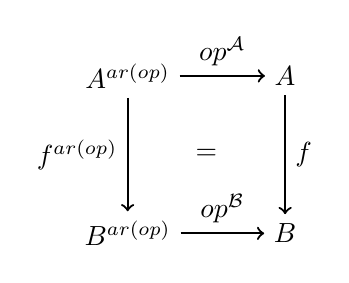
\begin{tikzpicture}
\node (srcA) at (0.0, 2.0) {$A^{ar(op)}$};
\node (trgA) at (2.0, 2.0) {$A$};
\node (srcB) at (0.0, 0.0) {$B^{ar(op)}$};
\node (trgB) at (2.0, 0.0) {$B$};

\node (eq) at (1.0, 1.0) {$=$};

\tikzset{mystyle/.style={->,thick}};  
\path (srcA) edge [mystyle] node[above]{$op^\ca$} (trgA);
\path (srcB) edge [mystyle] node[above]{$op^\cb$} (trgB);
\path (srcA) edge [mystyle] node[left]{$f^{ar(op)}$} (srcB);
\path (trgA) edge [mystyle] node[right]{$f$} (trgB);
\end{tikzpicture}
\end{center}
\end{definition}

\subsection{Duality of injective \& surjective functions}

\begin{definition}
An arrow $f: B \to C$ is \emph{monic} if, for any pair of arrows $g: A\to B$ and $h: A\to B$, $g;\! f = h;\! f$\footnote{Not sure how to write compositions, which convention to follow. } implies $g=h$.
\end{definition}

\begin{proposition}
In $\cat{Set}$, monic arrows are just the injective functions ($f(x) = f(x)$ implies $x=y$). 
\end{proposition}

\begin{proof}
  Let $f: B\to C$ be an injective function, and let $g,h: A\to B$ be such that $g;\! f = h;\! f$, but $g\neq h$. This means there is an element $a\in A$ for which $g(a) \neq h(a)$. But since $f$ is injective, $f(g(a))\neq f(h(a))$ which contradicts $g;\! f = h;\! f$. So $f$ is monic.

  Conversely, let $f: B \to C$ be monic. If it's not injective, there are distinct elements $b, b' \in B$ for which $f(b) = f(b')$. Let $A$ be a~singleton set $\{a\}$, and let $g: A\to B$ map $a$ to $b$ while $h: A\to B$ maps $a$ to $b'$. Then $f(g(a)) = f(h(a))$, contradicting the assumption that $f$ is monic. 
\end{proof}

\begin{definition}
An arrow $f: A\to B$ is \emph{epic} if, for any pairs of arrows $g: B\to C$ and $h: B\to C$, $f;\! g = f;\! h$ implies $g=h$. Epic is clearly dual to monic. 
\end{definition}

\begin{proposition}
In $\cat{Set}$, epic arrows are just the surjective functions. 
\end{proposition}

\begin{proof}
  nigga please
\end{proof}

Simply speaking: \begin{proposition} A $\Sigma$-homomorphism $f : \ca \to \cb$ is
\begin{description}
\item [monic] iff $f : A \to B$ is \textit{injective}
\begin{center}
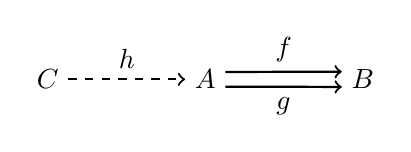
\begin{tikzpicture}
\node (A) at (-1.0, 0.0) {$A$};
\node (B) at (1.0, 0.0) {$B$};
\node (C) at (-3, 0) {$C$};

\tikzset{mystyle/.style={->,thick}};  
\path (A.20) edge [mystyle] node[above]{$f$} (B.160);
\path (A.340) edge [mystyle] node[below]{$g$} (B.200);
\tikzset{mystyle/.style={->,thick,dashed}};  
\path (C) edge[mystyle] node[above]{$h$} (A);
\end{tikzpicture}
\end{center}

\item [epic] iff $f : A \to B$ is \textit{surjective}
\begin{center}
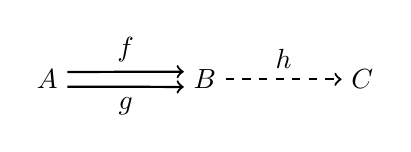
\begin{tikzpicture}
\node (A) at (-1.0, 0.0) {$A$};
\node (B) at (1.0, 0.0) {$B$};
\node (C) at (3, 0) {$C$};

\tikzset{mystyle/.style={->,thick}};  
\path (A.20) edge [mystyle] node[above]{$f$} (B.160);
\path (A.340) edge [mystyle] node[below]{$g$} (B.200);
\tikzset{mystyle/.style={->,thick,dashed}};  
\path (B) edge[mystyle] node[above]{$h$} (C);
\end{tikzpicture}
\end{center}

\item [iso] iff $f : A \to B$ is \textit{bijective}
\begin{center}
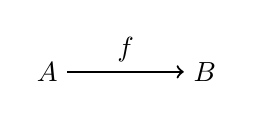
\begin{tikzpicture}
\node (A) at (-1.0, 0.0) {$A$};
\node (B) at (1.0, 0.0) {$B$};

\tikzset{mystyle/.style={->,thick}};  
\path (A) edge [mystyle] node[above]{$f$} (B);
\end{tikzpicture}
\end{center}
\end{description}
\end{proposition}

\section{Categories}

A \emph{category} $\acat{C}$ is a tuple comprising of:

\begin{enumerate}
\item a collection of \emph{objects};
\item a collection of \emph{morphisms} or \emph{arrows};
\item  operations assigning to each morphism $f$ a \emph{domain} $dom\ f$,
  and a \emph{codomain} $cod\ f$. We write $f: A \to B$ to show that
  $dom\ f = A$ and $cod\ f = B$. The collection of all arrows with
  domain $A$ and codomain $B$ is written $\acat{C}(A,B)$.
\item a composition operator assigning to each pair of arrows $f$ and $g$ a
  \emph{composite arrow} $g\circ f: dom\ f\to cod\ g$ that satisfies the
  law of associativity, i.e.~for any arrows $f: A \to B$, $g: B\to C$
  and $h: C \to D$: \[
  h\circ (g \circ f) = (h \circ g) \circ f
  \]
\item for each object $A$, an \emph{identity} arrow $id_A: A \to A$ that
  satisfies the identity law, i.e.~for any arrow $f: A\to B$:
  $id_B \circ f = f$ and $f\circ id_A = f$
\end{enumerate}

\textbf{Remark:} Collections mentioned above are meant in a
set-theoretical sense, i.e.~they are just sets or proper classes.

First we present a simple example, describing the category of sets.

\begin{example}Example: $\cat{Set}$

\begin{enumerate}
\item Objects in $\cat{Set}$ are sets.
\item Arrows $f: A\to B$ are total functions from set $A$ into set $B$.
\item For every total function $f$, its domain $A$ and codomain $B$, we get
  $dom\ f = A$, $cod\ f = B$, and $f \in \cat{Set}(A, B)$. \\\truls{Think it's written $f : \cat{Set}(A,B)$, isn't it?}
\item Composition of one total function $f: A\to B$ with another total
  function $g: B\to C$ is the total function from $A$ to $C$ mapping
  each element $a \in A$ to $g(f(a))\in C$. Composition of total
  functions on sets is associative: for any $f: A\to B$, $g: B\to C$ and
  $h:C \to D$, we get $h\circ (g\circ f) = (h\circ g)\circ f$.
\item For each set $A$, the identity function $id_A$ is a total function
  with domain and codomain $A$. For any function $f: A\to B$, the
  identity functions on $A$ and $B$ satisfy the equations required by
  the identity law: $id_B \circ f = f$ and $f \circ id_A = f$.
\end{enumerate}
\end{example}

\subsection{Dual notions}

For each category $\acat{C}$, the objects of the dual category $\acat{C}^{op}$ are the same as those in $\acat{C}$, but the arrows in $\cat{C}^{op}$ are opposite. If $f: A~\to B$ is an arrow of $\acat{C}$ then $f: B \to A$ is an arrow of $\acat{C}^{op}$.

\subsection{Initial \& final objects}

\begin{definition}
An object is called \emph{initial} if, for every object in $A$, there is exactly one arrow from it to $A$. 
\end{definition}

\begin{definition}
Dually, an object is \emph{terminal} if, for every object in $A$, there is exactly one arrow from $A$ to $1$. 
\end{definition}

In $\cat{Set}$, the empty set $\emptyset$ is the only initial object: for every set $S$, the empty function is the only function from $\emptyset$ to $S$.

Dually, each singleton set is a~terminal object, since for every set $S$ there is a~function from $S$ to a~singleton set $\{x\}$ mapping every element of $S$ to $x$, and this is the only total function from $S$ to $\{x\}$. 

\subsubsection{Cartesian products and disjoint unions}

\begin{itemize}
\item elements can be treated as arrows from a~terminal object
\item when we form a~product $A\times B$ we also define projections $\pi_{1}: A\times B \to A$ and $\pi_{2}: A\times B \to B$
\item so product is actually a~tuple $(A\times B, \pi_{1},\pi_{2})$.
\end{itemize}

Let $C$ be a~set and $f: C\to A$, $g: C\to B$. We say a~\emph{product function} $\langle f,g\rangle: C \to A\times B$ is
\[
\langle f, g\rangle (x) = (f(x), g(x))
\]
Functions $f$ and $g$ can be recovered from $\langle f, g\rangle$ by setting $f = \langle f,g\rangle;\! \pi_{1}$ and $g = \langle f, g\rangle;\! \pi_{2}$.

\begin{definition}
  A~\emph{product} of two objects $A$ and $B$ is an object $A\times B$ together with \emph{projection arrows} $\pi_{1}: A\times B \to A$ and $\pi_{2}: A\times B \to B$, such that for any object $C$ and pair of arrows $f: C\to A$ and $g: C\to B$ there is exactly one \emph{mediating} arrow $\langle f,g\rangle: C\to A\times B$ making the diagram
  
  \begin{center}
    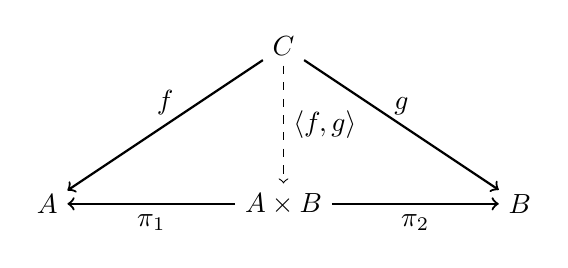
\begin{tikzpicture}
      \node (C)   at (0, 2) {$C$};
      \node (A)   at (-3, 0) {$A$};
      \node (B)   at (3, 0) {$B$};
      \node (AxB) at (0, 0) {$A\times B$};
      
      \tikzset{mystyle/.style={->,thick}};
 
      \path (AxB) edge [mystyle] node[below]{$\pi_{1}$} (A);
      \path (AxB) edge [mystyle] node[below]{$\pi_{2}$} (B);
      
      \path (C) edge[mystyle] node[left,above]{$f$} (A);
      \path (C) edge[mystyle] node[right,above]{$g$} (B);
      \tikzset{mystyle/.style={->,dashed}};
      \path (C) edge [mystyle] node[right]{$\langle f,g\rangle$} (AxB);
    \end{tikzpicture}
  \end{center}
  commute, i.e. $\langle f,g\rangle;\! \pi_{1} = f$ and $\langle f,g\rangle;\! \pi_{2} = g$.
\end{definition}

\begin{definition}
  A~\emph{coproduct} of $A$ and $B$ is $A+B$ together with two \emph{injection arrows} $c_{1}: A\to A+B$, $c_{2}: B \to A+B$, such that for any object $C$ and pair of arrows $f: A\to C$ and $g: B\to C$ there is exactly one arrow $[f,g]: A+B \to C$ making the diagram below commute.
  \begin{center}
    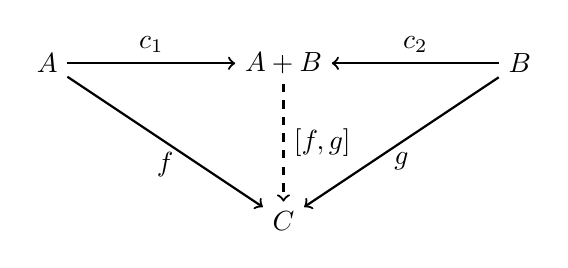
\begin{tikzpicture}
      \node (A)   at (-3, 0) {$A$};
      \node (A+B) at (0,0)   {$A+B$};
      \node (B)   at (3,0)   {$B$};
      \node (C)   at (0,-2)  {$C$};

      \tikzset{mystyle/.style={->,thick}};
      \path (A) edge [mystyle] node[above]{$c_{1}$} (A+B);
      \path (B) edge [mystyle] node[above]{$c_{2}$} (A+B);
      \path (A) edge [mystyle] node[left,below]{$f$} (C);
      \path (B) edge [mystyle] node[right,below]{$g$} (C);

      \tikzset{mystyle/.style={->,thick,dashed}};
      \path (A+B) edge [mystyle] node[right]{$[f,g]$} (C);
    \end{tikzpicture}
  \end{center}
  \emph{Remark:} $[f,g]$ is a~case distinction. 
\end{definition}

\subsection{Epi-mono factorization and the kernel}
For any map $f : A \to B$ there is an epi-mono factorization. That is there are
maps $f'_1 : A \to Z$ and $f'_2 : Z \to B$ such that
\begin{itemize}
\item $f'_1$ is epi,
\item $f'_2$ is mono, and
\item $f = f'_1;f'_2$.
\end{itemize}

\begin{proposition} Epi-mono factorizations are unique upto isomorphisms
  \begin{center}
    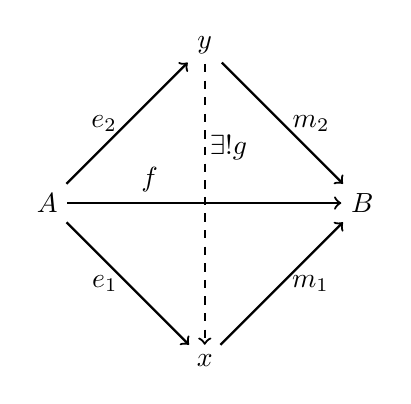
\begin{tikzpicture}
      \node (A) at (-2.0, 0.0) {$A$}; \node (B) at (2.0, 0.0) {$B$};

      \node (y) at (0, 2) {$y$}; \node (x) at (0, -2) {$x$};

      \node (f) at (-0.7, 0.3) {$f$}; \node (g) at (0.3, 0.7) {$\exists ! g$};

      \tikzset{mystyle/.style={->,thick}}; \path (A) edge [mystyle] node {} (B);
      \path (A) edge[mystyle] node[left]{$e_2$} (y); \path (A) edge[mystyle]
      node[left]{$e_1$} (x); \path (y) edge[mystyle] node[right]{$m_2$} (B);
      \path (x) edge[mystyle] node[right]{$m_1$} (B);
      \tikzset{mystyle/.style={->,thick,dashed}}; \path (y) edge[mystyle]
      node[right]{} (x);
    \end{tikzpicture}
  \end{center}
\end{proposition}

\begin{definition}\textbf{(Kernel)} The \textit{kernel} $ker(f)$ of a function
  is the relation
$$ker(f) = \{(a,a') \in A \times A ~|~ f(a) = f(a')\}$$
\end{definition}

The kernel of a function induces an equivalence on the domain
\begin{equation}
  \equiv ~:=~ ker(f)
\end{equation}

This allows the construction of the quotient set
\begin{equation}
  A/_\equiv ~:=~ \{[a]_\equiv ~|~ a \in A\} \text{ where } [a]_\equiv = \{a' ~|~ (a,a') \in \equiv\}
\end{equation}

\begin{center}
  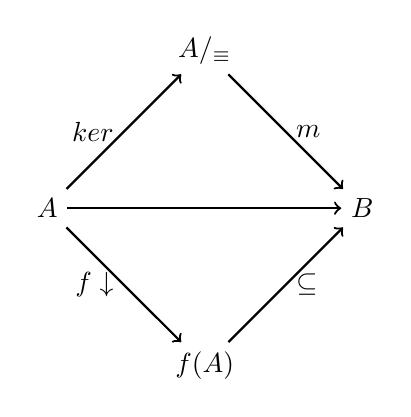
\begin{tikzpicture}
    \node (A) at (-2.0, 0.0) {$A$}; \node (B) at (2.0, 0.0) {$B$};

    \node (y) at (0, 2) {$A/_\equiv$}; \node (x) at (0, -2) {$f(A)$};

    \tikzset{mystyle/.style={->,thick}}; \path (A) edge [mystyle] node {} (B);
    \path (A) edge[mystyle] node[left]{$ker$} (y); \path (A) edge[mystyle]
    node[left]{$f\downarrow$} (x); \path (y) edge[mystyle] node[right]{$m$} (B);
    \path (x) edge[mystyle] node[right]{$\subseteq$} (B);
  \end{tikzpicture}
\end{center}

\begin{definition}\textbf{(Equ(A))} All equivalence classes on $A$ is $Equ(A)$.
\end{definition}

\begin{proposition} About $Equ(A)$
  \begin{itemize}
  \item $Equ(A)$ is ordered by $\subseteq$
    \begin{itemize}
    \item the minimal element is the diagonal $\Delta_A = \{(a,a) ~|~ a \in A\}$
    \item the maximal element is the complete graph $A\times A$
    \end{itemize}
  \item \textbf{meet:} Equ(A) is closed under intersection
  \item \textbf{join:} the join of $\equiv_1$ and $\equiv_2$ is the equivalence class $\equiv$
    generated by $\equiv_1 \cup \equiv_2$.
  \end{itemize}
\end{proposition}

\begin{definition}\textbf{($\Sigma$-conguence)} Let $\ca$ be an algebra. $\equiv ~\subseteq~ A^2$
  is a $\Sigma$-congruence if
  \begin{itemize}
  \item $\equiv$ is an equivalence relation on $A$, and
  \item for each $op \in OP$ with $n = ar(op)$
$$ \text{if } (a_1, a_1'), \dots , (a_n, a_n') \in \equiv \text{ then } (op^\ca(a_1, \dots, a_n), op^\ca(a_1', \dots, a_n')) \in \equiv$$
\end{itemize}
\end{definition}



\begin{definition}[Equalizer]
  \label{def:equalizer}
   An equalizer of two parallel morphisms $f, g : A \rightarrow B$
  in a category C consists of an object E and a morphism $m : E \rightarrow A$
  with $m; f = m; g$. Moreover, the pair $(E, m)$ satisfies the following universal
  property\footnote{This universal property essentially says that E must be as
    big as possible.}:
  \begin{itemize}
  \item For any other object X and morphism $f_x : X \rightarrow A$ with $f_{x} ; f = fx ;
    g$ there exists a unique morphism $k : X \rightarrow E$ such that $k; m =
    f_x$.
  \end{itemize}

  Picture:
      \xymatrix{
      X \ar@{.>}[d]_{\exists !k} \ar[dr]^{f_{x}} & & \\
      E \ar[r]^{m} & A \ar@/^/[r]^{f} \ar@/_/[r]_{g} & B}
  \end{definition}

\begin{proposition} If $f$ is a $\Sigma$-homomorphism, then $ker(f)$ is a
  $\Sigma$-congruence.
\end{proposition}

Categorically, the kernel is an equalizer of $\pi_1;f$ and $\pi_2;f$ (i.e., a pullback
of $(f,f)$) in the following diagram
\begin{center}
  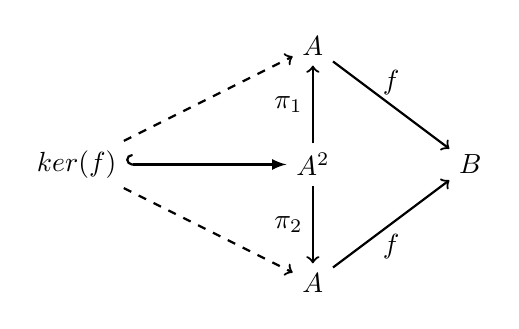
\begin{tikzpicture}
    \node (A) at (0.0, -1.5) {$A$}; \node (A') at (0, 1.5) {$A$}; \node (A2) at
    (0, 0) {$A^2$};

    \node (B) at (2.0, 0.0) {$B$}; \node (ker) at (-3, 0) {$ker(f)$};


    \tikzset{mystyle/.style={->,thick}}; \path (A) edge [mystyle]
    node[below]{$f$} (B); \path (A') edge [mystyle] node[above]{$f$} (B); \path
    (A2) edge[mystyle] node[left]{$\pi_2$} (A); \path (A2) edge[mystyle]
    node[left]{$\pi_1$} (A'); \tikzset{mystyle/.style={->,thick,dashed}}; \path
    (ker) edge[mystyle] node{} (A); \path (ker) edge[mystyle] node{} (A');
    \tikzset{mystyle/.style={->,thick,right hook-latex}}; \path (ker)
    edge[mystyle] node[above]{} (A2);
  \end{tikzpicture}
\end{center}

\section{Initial $\Sigma$-algebras}
\begin{minipage}[b]{0.4\linewidth}
\begin{center}
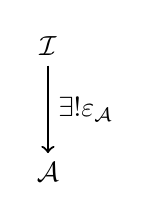
\begin{tikzpicture}
\node (I) at (0.0, 0.8) {$\mathcal I$};
\node (A) at (0.0, -0.8) {$\ca$};

\tikzset{mystyle/.style={->,thick}};  
\path (I) edge [mystyle] node[right]{$\exists!\varepsilon_\ca$} (A);
\end{tikzpicture}
\end{center}
\end{minipage}
\begin{minipage}[b]{0.5\linewidth}
For all $\Sigma$-algebras, there is a unique $\Sigma$-homomorphism, $\varepsilon_\ca : \mathcal I \to \ca$.\\
$\rightsquigarrow~$ \textit{ground term} $\Sigma$-algebra, $\tau_\Sigma$\\
\end{minipage}

\begin{definition}\textbf{(Ground terms)} For a given signature $\Sigma$, the \textit{ground terms} $\tau_\Sigma$ is the least set which satisfies\footnote{Terms (elements of the carrier set of the term algebra) are underlined.}
$$\text{if } \underline{t_1}, \dots, \underline{t_n} \in \tau_\Sigma \text{ and }ar(op) = n \text{ then } \underline{op(t_1, \dots, t_n)} \in \tau_\Sigma.$$
\end{definition}

\begin{definition}\textbf{(Term algebra)} The \textit{term algebra} for a signature $\Sigma$, is the algebra where the carrier set is the set of ground terms, and the operations are defined by
$$op^{\tau_\Sigma}(\underline{t_1}, \dots , \underline{t_n}) ~:=~ \underline{op(t_1, \dots, t_n)}.$$
\end{definition}



\begin{proposition}The term algebra is initial.
\end{proposition}

\begin{proof} Let $\ca$ be an arbitrary $\Sigma$-algebra.
\begin{center}
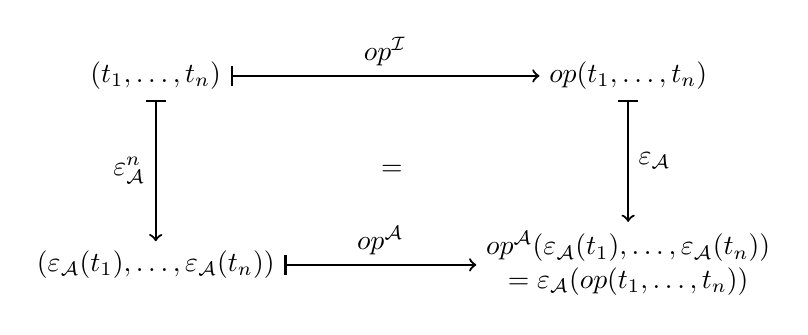
\begin{tikzpicture}
\node (nw) at (-3, 1.2) {$(t_1, \dots, t_n)$};
\node (ne) at (3, 1.2) {$op(t_1, \dots, t_n)$};
\node (sw) at (-3, -1.2) {$(\varepsilon_\ca(t_1), \dots, \varepsilon_\ca(t_n))$};
\node (se) at (3, -1.2) {$\begin{matrix}op^\ca(\varepsilon_\ca(t_1), \dots, \varepsilon_\ca(t_n))\\=\varepsilon_\ca(op(t_1, \dots, t_n))\end{matrix}$};
\node (eq) at (0, 0) {$=$};

\tikzset{mystyle/.style={|->,thick}};  
\path (nw) edge [mystyle] node[left]{$\varepsilon_\ca^n$} (sw);
\path (nw) edge [mystyle] node[above]{$op^{\mathcal I}$} (ne);
\path (ne) edge [mystyle] node[right]{$\varepsilon_\ca$} (se);
\path (sw) edge [mystyle] node[above]{$op^\ca$} (se);
\end{tikzpicture}
\end{center}
\end{proof}

\subsection{Characterization of Initial $\Sigma$-algebras}
\begin{itemize}
\item all $op^{\mathcal I}$ are injective
\item for all $op_1 \neq op_2$
$$op^{\mathcal I}_1(\underbrace{I^{ar(op_1)}}_{(*)}) \cap op^{\mathcal I}_2(\underbrace{I^{ar(op_2)}}_{(*)}) = \emptyset.$$
$(*)$ is a vector of appropriate arguments
\item for all $i \in I$ there exists $op \in OP$ and $i_1, \dots, i_n \in I$ such that
$$ op(i_1, \dots, i_n) = i.$$
\item $\mathcal I$ has no propper subalgebras
\end{itemize}

\section{Functors}

\begin{definition}[Functor]
  Let $\acat{C}$ and $\acat{D}$ be any categories. A~\emph{functor} $F: \acat{C} \to \acat{D}$ is a~map that takes each $\acat{C}$-object $A$ to a~$\acat{D}$-object $F(A)$ and each $\acat{C}$-arrow $f: A\to B$ to a~$\acat{D}$-arrow $F(f): F(A) \to F(B)$, such that for all $\acat{C}$-objects $A$ and composable $\acat{C}$-arrows $f$ and $g$:
  \begin{enumerate}
  \item $F(id_{A}) = id_{F(A)}$
  \item $F(f;\! g) = F(f);\! F(g)$.
  \end{enumerate}
\end{definition}

Some examples of functors:

\textbf{Constant functor (aka \emph{selection} functor)} is a~functor $Cd: \acat{C} \to \acat{D}$ that maps every object of $\acat{C}$ to a~fixed object $d$ in $\acat{D}$ and every morphism in $\acat{C}$ to the identity morphism on $d$.

\textbf{Diagonal functor} $\Delta: \acat{C} \to \acat{C} \times \acat{C}$ takes each object $A$ of $\acat{C}$ to the object $(A,A)$ in the product category $\acat{C}\times\acat{C}$. Example of a~diagonal functor looks like this:
\begin{center}
  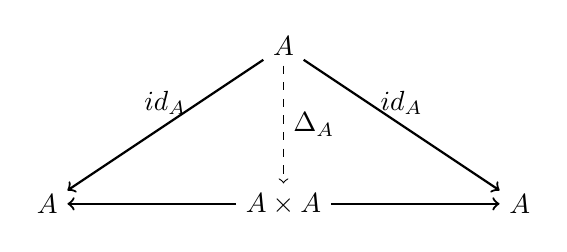
\begin{tikzpicture}
    \node (C)   at (0, 2) {$A$};
    \node (A)   at (-3, 0) {$A$};
    \node (B)   at (3, 0) {$A$};
    \node (AxB) at (0, 0) {$A\times A$};
    
    \tikzset{mystyle/.style={->,thick}};
 
    \path (AxB) edge [mystyle]  (A);
    \path (AxB) edge [mystyle]  (B);
      
    \path (C) edge[mystyle] node[left,above]{$id_{A}$} (A);
    \path (C) edge[mystyle] node[right,above]{$id_{A}$} (B);
    \tikzset{mystyle/.style={->,dashed}};
    \path (C) edge [mystyle] node[right]{$\Delta_{A}$} (AxB);
  \end{tikzpicture}
\end{center}
where $\Delta_{A} = \langle id_{A},id_{A}\rangle$.

\textbf{Product functor} is a~functor $\times: \acat{C} \times \acat{C} \to \acat{C}$. It looks something like this:
\begin{center}
  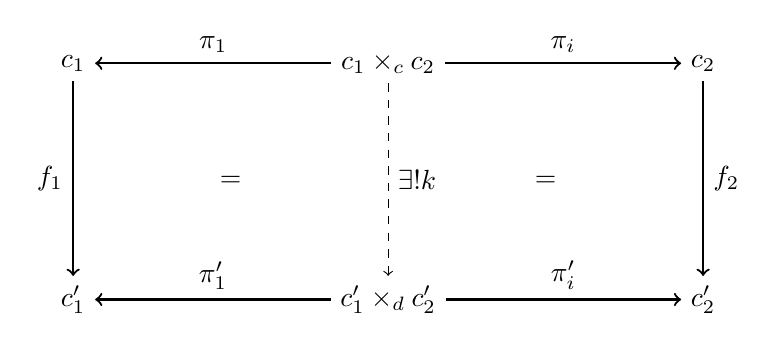
\begin{tikzpicture}
    \node (c1xcc2) at (0, 0) {$c_{1} \times_{c} c_{2}$};
    \node (c1) at (-4, 0) {$c_{1}$};
    \node (c2) at (4, 0) {$c_{2}$};

    \node (c1pxdc2p) at (0, -3) {$c_{1}' \times_{d} c_{2}'$};
    \node (c1p) at (-4, -3) {$c_{1}'$};
    \node (c2p) at (4, -3) {$c_{2}'$};

    \node (eq1) at (2, -1.5) {$=$};
    \node (eq2) at (-2, -1.5) {$=$};

    \tikzset{mystyle/.style={->,dashed}};  
    \path (c1xcc2) edge[mystyle] node[right]{$\exists ! k$} (c1pxdc2p);

    \tikzset{mystyle/.style={->,thick}};
    \path (c1xcc2) edge [mystyle] node[above]{$\pi_1$} (c1);
    \path (c1xcc2) edge [mystyle] node[above]{$\pi_i$} (c2);
    \path (c1pxdc2p) edge [mystyle] node[above]{$\pi_1'$} (c1p);
    \path (c1pxdc2p) edge [mystyle] node[above]{$\pi_i'$} (c2p);
    \path (c1) edge[mystyle] node[left]{$f_{1}$} (c1p);
    \path (c2) edge[mystyle] node[right]{$f_{2}$} (c2p);
  \end{tikzpicture}
\end{center}
where $k = \langle \pi_{1};\! f, \pi_{i};\! f_{i}\rangle = f_{1}\times f_{2}$.

\textbf{Powerset functor(s)}. Ok, hold tight. We say that a~\emph{powerset functor} is such a~functor $P: \cat{Set} \to \cat{Set}$ that maps each set to its power set and each function $f: X \to Y$ to the map which sends $U \subseteq X$ to its image $f(U) \subseteq Y$. Then a~\emph{covariant powerset} functor is such a~functor $G: \cat{Set} \to \cat{Set}$ that maps each function $f: A \to B$ into $G(f): G(A) \to G(B)$ which is defined by $G(f)(X) = f(X)$ for any $X \subseteq A$. Also, a~\emph{contravariant powerset} functor is such a~functor $H: \cat{Set} \to \cat{Set}$ that sends $f: X \to Y$ to the map which sends $V \subseteq Y$ to its inverse image $f^{-1} (V) \subseteq X$. 

\textbf{Function space functor} looks like this:

\begin{minipage}{0.45\textwidth}
  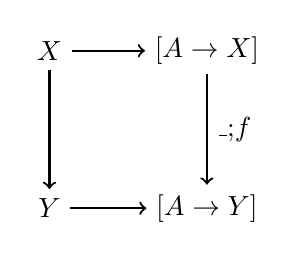
\begin{tikzpicture}
    \node (x)    at (0, 0)   {$X$};
    \node (atox) at (2, 0)   {$[A \to X]$};
    \node (y)    at (0,-2)   {$Y$};
    \node (atoy) at (2,-2)   {$[A \to Y]$};

    \tikzset{mystyle/.style={->,thick}};
    \path (x) edge [mystyle] (atox);
    \path (x) edge [mystyle] (y);
    \path (y) edge [mystyle] (atoy);
    \path (atox) edge [mystyle] node[right]{$\_;\! f$} (atoy);
  \end{tikzpicture}
\end{minipage}
\begin{minipage}{0.45\textwidth}
where $\_;\! f$ is a~composition like this:
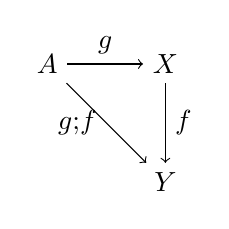
\begin{tikzpicture}
  \node (A) at (0,0) {$A$};
  \node (X) at (1.5,0) {$X$};
  \node (Y) at (1.5,-1.5) {$Y$};
  \tikzset{mystyle/.style={->}};
  \path (A) edge[mystyle] node[above] {$g$} (X);
  \path (X) edge[mystyle] node[right] {$f$} (Y);
  \path (A) edge[mystyle] node[below,left] {$g;\! f$} (Y);
\end{tikzpicture}
\end{minipage}

\section{Induction $\simeq$ Initiality ($\simeq$ Universal property of Constructors)}
\truls{This section has eroded in to ramblings. I'm tired and I don't think I understand this anymore.}

Consider some signature $\Sigma = (OP, ar)$. We have some basic vocabulary (constants and operations) to describe stuff. Suppose that we would like to define some function over these things. Standard structural induction of some function $f$ in this vocabulary goes about first defining the value of $f$ for all the constants and then how $f$ changes when we apply operations to the arguments of $f$.

Say we have two constants ($c_1$ and $c_2$) and one unary operator ($u$). Our induction scheme would be 
\begin{align*}
f(c_1) &= \dots & \text{Base case 1} \\
f(c_2) &= \dots & \text{Base case 2} \\
f(u(x)) &= \dots(f(\dots)) & \text{Induction step}
\end{align*}

This should 
\begin{enumerate}
\item Define $f$ uniquely, and
\item Define $f$ completely.
\end{enumerate}

Or, in other words
\begin{enumerate}
\item if both $f$ and $g$ complies with the definition, then\footnote{Upto isomorphism.} $f = g$, and \\
(uniqueness of homomorphism from initial object)
\item For every $x$, $f(x)$ is well-defined.\\
(the initial algebra has no proper subalgebras)
\end{enumerate}

Structurally we can define a function as an algebra, and the inductive definition of the function described by the algebra will just be a homomorphism from the initial object to this given algebra. 

\begin{example} Let $\Sigma_{\mathcal N} = (OP_{\mathcal N}, ar_{\mathcal N}) = (\{0, s\}, \{(0, 0), (s, 1)\})$ be the signature of the natural numbers. The initial algebra is the term-algebra $\mathcal I_{\mathcal N} = (\nn; 0, s)$ where we take $\nn$ to be the set of ground terms $\{0, s0, ss0, sss0, \dots\}$. 

Suppse we would like to define some function $f$ which, in the classical notation would be defined as follows\footnote{I tried to make $f(sx) := g(f(h(x)))$, but I'm not sure of how to handle the $h$ yet... \\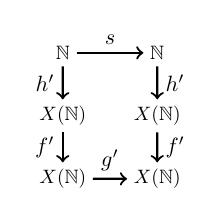
\begin{tikzpicture}[scale=0.4]
\node[scale=0.7] (a1) at (-1, 1) {$\nn$};
\node[scale=0.7] (a2) at (2, 1) {$\nn$};
\node[scale=0.7] (b1) at (-1, -1) {$X(\nn)$};
\node[scale=0.7] (b2) at (2, -1) {$X(\nn)$};
\node[scale=0.7] (c1) at (-1, -3) {$X(\nn)$};
\node[scale=0.7] (c2) at (2, -3) {$X(\nn)$};

\tikzset{mystyle/.style={->,thick}};  
\path (a1) edge [mystyle] node[above, scale=0.8]{$s$} (a2);
\path (a1) edge [mystyle] node[left, scale=0.8]{$h'$} (b1);
\path (a2) edge [mystyle] node[right, scale=0.8]{$h'$} (b2);
\path (b1) edge [mystyle] node[left, scale=0.8]{$f'$} (c1);
\path (b2) edge [mystyle] node[right, scale=0.8]{$f'$} (c2);
\path (c1) edge [mystyle] node[above, scale=0.8]{$g'$} (c2);
\end{tikzpicture} and then some $l$ such that
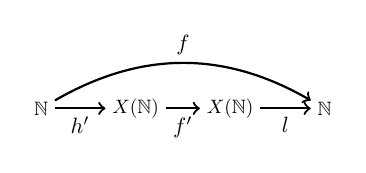
\begin{tikzpicture}[scale=0.4]
\node[scale=0.7] (a) at (0, 0) {$\nn$};
\node[scale=0.7] (b) at (3, 0) {$X(\nn)$};
\node[scale=0.7] (c) at (6, 0) {$X(\nn)$};
\node[scale=0.7] (d) at (9, 0) {$\nn$};

\tikzset{mystyle/.style={->,thick}};  
\path (a) edge [mystyle] node[below, scale=0.8]{$h'$} (b);
\path (b) edge [mystyle] node[below, scale=0.8]{$f'$} (c);
\path (c) edge [mystyle] node[below, scale=0.8]{$l$} (d);
\path (a) edge [mystyle, bend left] node[above, scale=0.8]{$f$} (d);
\end{tikzpicture}or something crazy like that...}: 
\begin{align*}
f(0) ~&:=~ c & \text{Base case}\\
f(sx) ~&:=~ g(f(x)) & \text{Induction step}
%f(sx) ~&:=~ g(f(h(x))) & \text{Induction step}
\end{align*}
where $h$ is some previously defined function over $\mathcal I_{\mathcal N}$. 

Now, suppose I provide two diagrams: 
\begin{figure}[ht]
\begin{minipage}[b]{0.4\linewidth}
\begin{center}
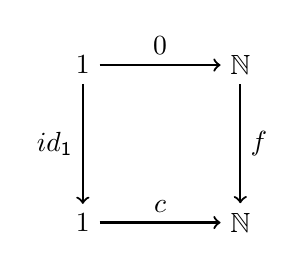
\begin{tikzpicture}
\node (a1) at (-1, 1) {$\mathbbm 1$}; % Truls dear, is this what you wanted?
\node (a2) at (1, 1) {$\nn$};
\node (b1) at (-1, -1) {$\mathbbm 1$};
\node (b2) at (1, -1) {$\nn$};

\tikzset{mystyle/.style={->,thick}};  
\path (a1) edge [mystyle] node[above]{$0$} (a2);
\path (a1) edge [mystyle] node[left]{$id_{\mathsf 1}$} (b1);
\path (b1) edge [mystyle] node[above]{$c$} (b2);
\path (a2) edge [mystyle] node[right]{$f$} (b2);
\end{tikzpicture}
\end{center}
\end{minipage}
\begin{minipage}[b]{0.4\linewidth}
\begin{center}
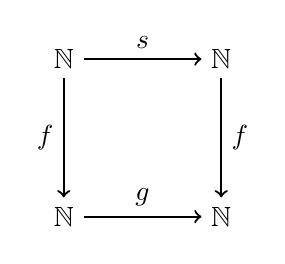
\begin{tikzpicture}
\node (a1) at (-1, 1) {$\nn$};
\node (a2) at (1, 1) {$\nn$};
\node (b1) at (-1, -1) {$\nn$};
\node (b2) at (1, -1) {$\nn$};

\tikzset{mystyle/.style={->,thick}};  
\path (a1) edge [mystyle] node[above]{$s$} (a2);
\path (a1) edge [mystyle] node[left]{$f$} (b1);
\path (b1) edge [mystyle] node[above]{$g$} (b2);
\path (a2) edge [mystyle] node[right]{$f$} (b2);
\end{tikzpicture}
\end{center}
\end{minipage}
\end{figure}

Recall that $c$ is some constant expression in $\mathcal I_{\mathcal N}$ and $g$ is a function in it. If I now say that $f$ is the map which makes both of these diagrams commute, we have defined $f$. 

We have that $f : \nn \to \nn$, but also that it is the map in a homomorphism from $\mathcal I_{\mathcal N}$ to $\ca_f$ where $\ca_f = (f(\nn); c, g)$. We can see that, treated as a homomorphism in $\cat{Alg}(\Sigma)$, it maps $n : \mathcal I_{\mathcal N}$ to $f(n) : \ca_f$.
\end{example}


\begin{example}Let's define the function $2 * \_ : \nn \to \nn$! 
\begin{description}
\item[Old school] Base case: $2 * 0 := 0$; induction step: $2 * s(n) := (2 * n) + 2$.
\item[21st century] ``Make it communte!'' (Paraphrasing Tom Waits)
\begin{figure}[ht]
\begin{minipage}[b]{0.4\linewidth}
\begin{center}
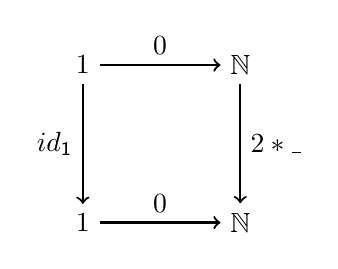
\begin{tikzpicture}
\node (a1) at (-1, 1) {$\mathbbm 1$};
\node (a2) at (1, 1) {$\nn$};
\node (b1) at (-1, -1) {$\mathbbm 1$};
\node (b2) at (1, -1) {$\nn$};

\tikzset{mystyle/.style={->,thick}};  
\path (a1) edge [mystyle] node[above]{$0$} (a2);
\path (a1) edge [mystyle] node[left]{$id_{\mathsf 1}$} (b1);
\path (b1) edge [mystyle] node[above]{$0$} (b2);
\path (a2) edge [mystyle] node[right]{$2 * \_$} (b2);
\end{tikzpicture}
\end{center}
\caption{\\Base case}
\end{minipage}
\begin{minipage}[b]{0.4\linewidth}
\begin{center}
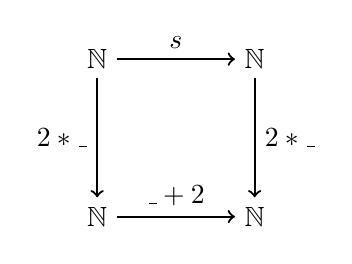
\begin{tikzpicture}
\node (a1) at (-1, 1) {$\nn$};
\node (a2) at (1, 1) {$\nn$};
\node (b1) at (-1, -1) {$\nn$};
\node (b2) at (1, -1) {$\nn$};

\tikzset{mystyle/.style={->,thick}};  
\path (a1) edge [mystyle] node[above]{$s$} (a2);
\path (a1) edge [mystyle] node[left]{$2 * \_$} (b1);
\path (b1) edge [mystyle] node[above]{$\_ + 2$} (b2);
\path (a2) edge [mystyle] node[right]{$2 * \_$} (b2);
\end{tikzpicture}
\end{center}
\caption{\\Induction step}
\end{minipage}
\end{figure}

Observe:
\begin{itemize}
\item The \textit{induction schema} is always the same (that's just the homomorphism property)
\item Only the ``constants'' and operations changes ($\rightsquigarrow ~ \Sigma$-algebra)
\end{itemize}
\end{description}
\end{example}

\begin{example} What is $2 * 2$?
\begin{center}
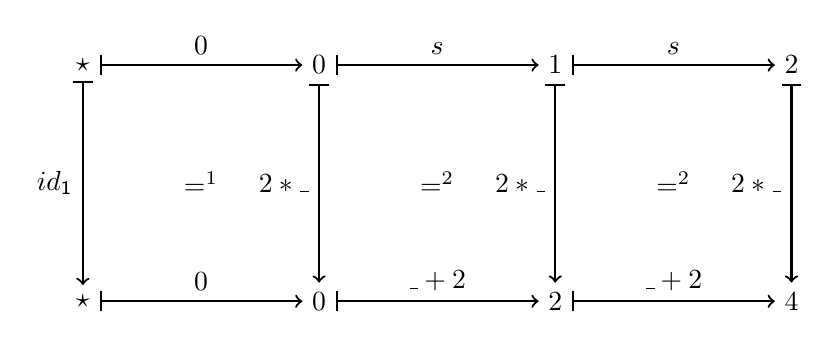
\begin{tikzpicture}
\node (s) at (0, 1) {$\star$};
\node (s') at (0, -2) {$\star$};
\node (f1) at (1.5, -0.5) {$=^1$};

\node (0) at (3, 1) {$0$};
\node (0') at (3, -2) {$0$};
\node (f1) at (4.5, -0.5) {$=^2$};

\node (1) at (6, 1) {$1$};
\node (1') at (6, -2) {$2$};
\node (f1) at (7.5, -0.5) {$=^2$};

\node (2) at (9, 1) {$2$};
\node (2') at (9, -2) {$4$};

\tikzset{mystyle/.style={|->,thick}};  
\path (s) edge [mystyle] node[above]{$0$} (0);
\path (0) edge [mystyle] node[above]{$s$} (1);
\path (1) edge [mystyle] node[above]{$s$} (2);

\path (s) edge[mystyle] node[left]{$id_{\mathsf 1}$} (s');
\path (0) edge[mystyle] node[left]{$2 * \_$} (0');
\path (1) edge[mystyle] node[left]{$2 * \_$} (1');
\path (2) edge[mystyle] node[left]{$2 * \_$} (2');

\path (s') edge [mystyle] node[above]{$0$} (0');
\path (0') edge [mystyle] node[above]{$\_ + 2$} (1');
\path (1') edge [mystyle] node[above]{$\_ + 2$} (2');
\end{tikzpicture}
\end{center}
$=^1$ is given by the base case in our definition (Figure 1) and $=^2$ is given by the induction step (Figure 2).
So $2 * 2 = 4$.
\end{example}

\section{Abstraction step : describe an algebra as a single arrow}
A signature $\Sigma$ corresponds to a (type) functor $T_\Sigma : \mathsf{Set} \to \mathsf{Set}$. A $\Sigma$-\textit{algebra} $\ca$ with carrier set $A$, corresponds to a map $\alpha : T_\Sigma(A) \to A$. \truls{Need more? Didn't write down the general definition. Could invent it, but not completely sure where I'd stick the parameters if there are any.}

\section{Categories}
We abstract.

\subsection{$\mathsf{Alg}(T_\Sigma) \cong \mathsf{Alg}(\Sigma)$}

Each $T_\Sigma$-algebra $(\alpha, A)$ defines a $\Sigma$-algebra $\ca_\alpha$ with carrier $A$ and operations $op^{\ca_\alpha} = x_i;\alpha$. 

\begin{proposition} $\ca_{\alpha_\ca} = \ca$
\end{proposition}

\begin{proof} 1 and 2
\begin{enumerate}
\item $\ca \mapsto (\alpha_\ca, A) \mapsto \ca_{\alpha_\ca} = \ca$
\item $(\alpha, A) \mapsto \ca_\alpha \mapsto (\alpha_{\ca_\alpha}, A) = (\alpha, A)$
\end{enumerate}

\end{proof}

\subsection{Algebras and Limits}
Let $T$ be an endofunctor in category $\mathbb C$. Then $Alg(T)$ is the category of algebras of that type. 

\begin{proposition} $\mathsf{Alg}(T)$ inherits all limits from $\mathbb C$.
\end{proposition}

Limits in $\mathsf{Alg}(T)$ are constructed by the limits on the \textit{carrier} from $\mathbb C$.

\begin{example} We illustrate the previous proposition with \textit{product}.

\begin{figure}[ht]
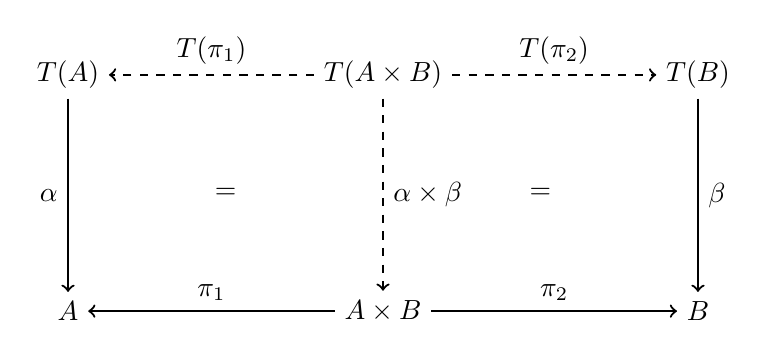
\begin{tikzpicture}
\node (tab) at (0, 0) {$T(A \times B)$};
\node (ta) at (-4, 0) {$T(A)$};
\node (tb) at (4, 0) {$T(B)$};

\node (ab) at (0, -3) {$A \times B$};
\node (a) at (-4, -3) {$A$};
\node (b) at (4, -3) {$B$};

\node (eq1) at (2, -1.5) {$=$};
\node (eq2) at (-2, -1.5) {$=$};

\tikzset{mystyle/.style={->,thick,dashed}};  
\path (tab) edge [mystyle] node[above]{$T(\pi_1)$} (ta);
\path (tab) edge [mystyle] node[above]{$T(\pi_2)$} (tb);
\path (tab) edge[mystyle] node[right]{$\alpha \times \beta$} (ab);

\tikzset{mystyle/.style={->,thick}};  
\path (ab) edge [mystyle] node[above]{$\pi_1$} (a);
\path (ab) edge [mystyle] node[above]{$\pi_2$} (b);
\path (ta) edge[mystyle] node[left]{$\alpha$} (a);
\path (tb) edge[mystyle] node[right]{$\beta$} (b);
\end{tikzpicture}
\caption{$\alpha \times \beta ~:=~ \langle T(\pi_1);\alpha, T(\pi_2);\beta \rangle$ }
\end{figure}
\end{example}

(``limits/products are easy for algebras, \textit{because} the carrier is isolated on the RHS.'')

\begin{proposition} If $\mathbb C$ is a category with (an?) initial object and colimits of ascending chains and $T$ is an endofunctor in $\mathbb C$ which preserves colimits of ascending chains, then the category $\mathsf{Alg}(T)$ has (an?) initial object.
\end{proposition}

\section{Coalgebras $\cong$ systems with ``next-state semantics''}
Here are some coalgebras, which are of the form $A \to T(A)$ (turn the arrow). 

\begin{example} Examples of coalgebras. (Exercise: Describe the systems with words.)
\begin{enumerate}
\item $T(X) = X$, hence $\alpha : X \to T(X)$.
\item $T(X) = X + \mathsf 1$
\item $T(X) = X \times A$ ($A$ is just a parameter (e.g., a set of symbols))
\item $T(X) = X \times A + \mathsf 1$
\item $T(X) = [A \to X]$ ($[A \to X] \cong X^A$ (maps from $A$ to $X$))
\item $T(X) = \wp(X)$
\end{enumerate}
\end{example}

The category of $T$-coalgebras are denoted $\mathsf{CAlg}(T)$.

\begin{proposition} Let $T$ be an endofuctor in $\mathbb C$. $\mathsf{CAlg}(T)$ inherits all \textit{colimits} from $\mathbb C$.
\end{proposition}

\begin{example}The example of \textit{sum} would be basically the same the the example of \textit{product} above, but with the arrows going the other way.
\end{example}

\begin{example}Let $T(X) = X$. Coalgebras in $\mathsf{CAlg}(T)$ are of the form $\alpha : X \to X$. Given a state $x \in X$, we ``transition'' deterministically and unabiguously into the next state $\alpha(x) \in X$.
\begin{figure}[ht]
\begin{minipage}[b]{0.3\linewidth}
\begin{center}
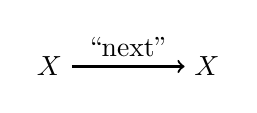
\begin{tikzpicture}
\node (xl) at (0, 0) {$X$};
\node (xr) at (2, 0) {$X$};

\tikzset{mystyle/.style={->,thick}};  
\path (xl) edge[mystyle] node[above]{``next''} (xr);
\end{tikzpicture}
\end{center}
\caption{``Shape''}
\end{minipage}
\begin{minipage}[b]{0.3\linewidth}
\begin{center}
\begin{tikzpicture}[scale=0.7]
\node (x1) at (0, 0) {$\cdot$};
\node (x2) at (-1, 1) {$\cdot$};
\node (x3) at (-1, -1) {$\cdot$};
\node (x4) at (-2.5, -1) {$\cdots$};
\node (x5) at (-2.5, 1) {$\cdots$};
\node (x6) at (1.5, 0) {$\cdots$};

\tikzset{mystyle/.style={->,thick}};  
\path (x1) edge[mystyle] node[]{} (x6);

\path (x2) edge[mystyle] node[above]{} (x1);
\path (x5) edge[mystyle] node[above]{} (x2);

\path (x3) edge[mystyle] node[above]{} (x1);
\path (x4) edge[mystyle] node[above]{} (x3);
\end{tikzpicture}
\end{center}
\caption{\\Arbitrary}
\end{minipage}
\begin{minipage}[b]{0.3\linewidth}
\begin{center}
\begin{tikzpicture}
\node (x) at (0, 0) {$\cdot$};

\tikzset{mystyle/.style={->,thick}};  
\path (x.0) edge[mystyle] node[bend right]{} (x.90);
\end{tikzpicture}
\end{center}
\caption{\\Final}
\end{minipage}
\end{figure}
\end{example}
\truls{The ``Final'' one above should just be a reflexive point. Don't know tikzpicture well enough to do that.}

\subsection{Discussion}
Recall (and extrapolate): 
\begin{itemize}
\item initial algebra $\cong$ induction. Dually, final coalgebra $\cong$ coinduction.
\item elements of initial algebra: (ground) terms; elements of final coalgebra: process/language/observable behaviour of systems.
\item ``final'' $\rightsquigarrow$ ``identify (``collapse'') as much as possible''. Need a way to ``avoid trivial collapse'': two elements/states in the final coalgebra are different if they can be distinguished by \textit{observations}. (Think \textit{bisimulation}!)
\end{itemize}

\subsection{Constructing the final coalgebra.} But first recall:
\subsubsection{Constructing the initial algebra $T^*(\mathcal I)$}
For simplicity assume that $T : \mathsf{Set} \to \mathsf{Set}$. Then $\mathcal I = \emptyset$. We start with an empty set of terms $\emptyset$, then construct all terms of ``complexity'' at most 1, then all terms of ``complexity'' at most 2, and so on. We collect these in the colimit, the set of all (reachable/ground) terms. See Figure (number).

\begin{figure}[ht]
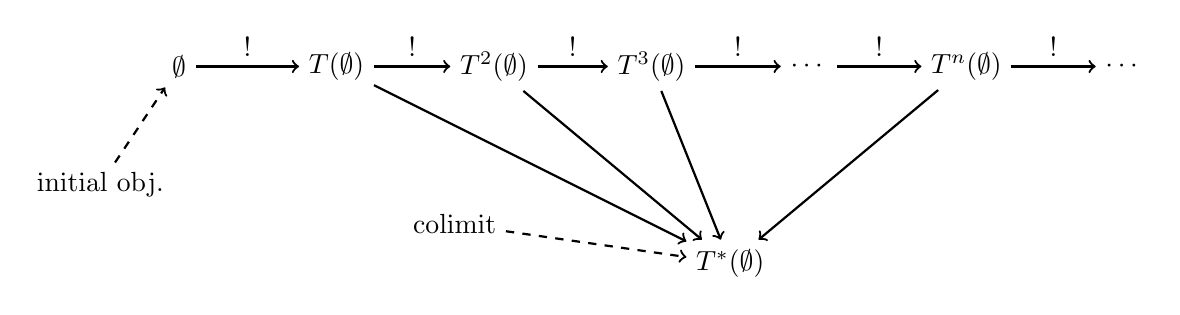
\begin{tikzpicture}
\node (01) at (0, 0) {$\emptyset$};
\node (02) at (2, 0) {$T(\emptyset)$};
\node (03) at (4, 0) {$T^2(\emptyset)$};
\node (04) at (6, 0) {$T^3(\emptyset)$};
\node (05) at (8, 0) {$\cdots$};
\node (06) at (10, 0) {$T^n(\emptyset)$};
\node (07) at (12, 0) {$\cdots$};

\node (star) at (7, -2.5) {$T^*(\emptyset)$};

\node (t1) at (-1, -1.5) {initial obj.};
\node (t2) at (3.5, -2) {colimit};

\tikzset{mystyle/.style={->,thick}};  
\path (01) edge[mystyle] node[above]{!} (02);
\path (02) edge[mystyle] node[above]{!} (03);
\path (03) edge[mystyle] node[above]{!} (04);
\path (04) edge[mystyle] node[above]{!} (05);
\path (05) edge[mystyle] node[above]{!} (06);
\path (06) edge[mystyle] node[above]{!} (07);

\path (02) edge[mystyle] node[above]{} (star);
\path (03) edge[mystyle] node[above]{} (star);
\path (04) edge[mystyle] node[above]{} (star);
\path (06) edge[mystyle] node[above]{} (star);

\tikzset{mystyle/.style={->,thick,dashed}};  
\path (t1) edge[mystyle] node[above, bend left]{} (01);
\path (t2) edge[mystyle] node[above, bend left]{} (star);
\end{tikzpicture}
\caption{Constructing the initial algebra.}
\end{figure}

Now, to construct the final coalgebra:\\

\begin{figure}[ht]
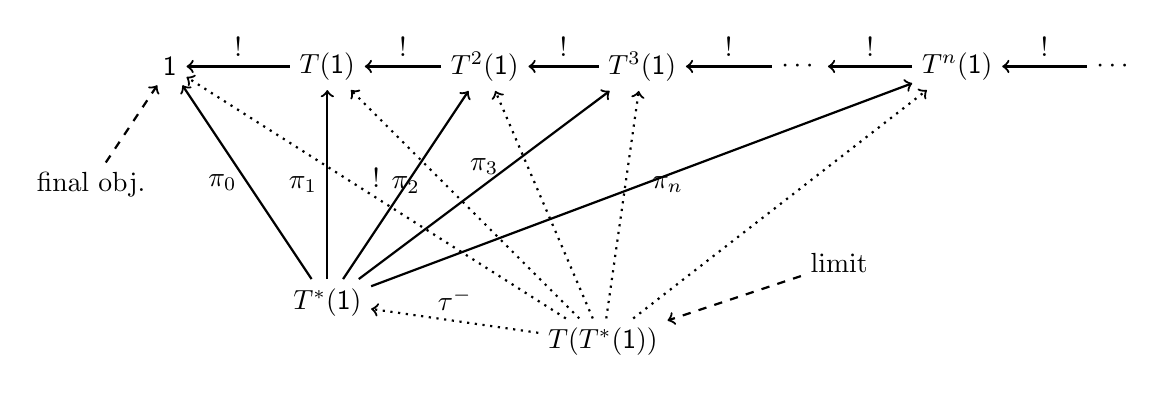
\begin{tikzpicture}
\node (01) at (0, 0) {$\mathsf 1$};
\node (02) at (2, 0) {$T(\mathsf 1)$};
\node (03) at (4, 0) {$T^2(\mathsf 1)$};
\node (04) at (6, 0) {$T^3(\mathsf 1)$};
\node (05) at (8, 0) {$\cdots$};
\node (06) at (10, 0) {$T^n(\mathsf 1)$};
\node (07) at (12, 0) {$\cdots$};

\node (star1) at (2, -3) {$T^*(\mathsf 1)$};
\node (star2) at (5.5, -3.5) {$T(T^*(\mathsf 1))$};

\node (t1) at (-1, -1.5) {final obj.};
\node (t2) at (8.5, -2.5) {limit};

\tikzset{mystyle/.style={->,thick}};  
\path (02) edge[mystyle] node[above]{!} (01);
\path (03) edge[mystyle] node[above]{!} (02);
\path (04) edge[mystyle] node[above]{!} (03);
\path (05) edge[mystyle] node[above]{!} (04);
\path (06) edge[mystyle] node[above]{!} (05);
\path (07) edge[mystyle] node[above]{!} (06);

\path (star1) edge[mystyle] node[left]{$\pi_0$} (01);
\path (star1) edge[mystyle] node[left]{$\pi_1$} (02);
\path (star1) edge[mystyle] node[]{$\pi_2$} (03);
\path (star1) edge[mystyle] node[above]{$\pi_3$} (04);
\path (star1) edge[mystyle] node[right]{$\pi_n$} (06);

\tikzset{mystyle/.style={->,thick,dotted}};  
\path (star2) edge[mystyle] node[above]{!} (01);
\path (star2) edge[mystyle] node[above]{} (02);
\path (star2) edge[mystyle] node[above]{} (03);
\path (star2) edge[mystyle] node[above]{} (04);
\path (star2) edge[mystyle] node[above]{} (06);

\path (star2) edge[mystyle] node[above]{$\tau^-$} (star1);

\tikzset{mystyle/.style={->,thick,dashed}};  
\path (t1) edge[mystyle] node[above, bend left]{} (01);
\path (t2) edge[mystyle] node[above, bend left]{} (star2);
\end{tikzpicture}
\caption{Constructing the initial algebra.}
\end{figure}

\truls{I don't know. I don't get it anymore.}

There is a unique $\tau^- : T(T^*(\mathsf 1)) \to T^*(\mathsf 1)$ such that $\tau^-;\pi_i = T(\pi_{i - 1})$. 

We still need $\tau : T_*(\mathsf 1) \to T(T_*(\mathsf 1))$. 

\truls{Could someone descripbe this process?}

\section{Modal Logic}
\newcommand{\bisim}{\,\underline{\leftrightarrow}\,}
\newcommand{\cam}{\mathcal M}
\newcommand{\prop}{\mathcal P}
\newcommand{\ff}{\mathcal F}
\newcommand{\xx}{\mathcal X}
\newcommand{\iso}{\simeq}

\newcommand{\mm}{\mathcal M}
\newcommand{\eqcl}[1]{[\![#1]\!]}
\newcommand{\meq}{\leftrightsquigarrow}
\renewcommand{\qedsymbol}{\begin{large}$\ddot\circ$\end{large}}

\subsection{History \& Background}
$rain~;~rain\to wet~/~ \therefore wet$. ``Might rain tomorrow'': two \textit{modalities}  (treat as one now) (modality is a linguistic thing: relativizes the way we evaluate the truth of a statement): $\bullet$ \textit{alethic} and $\bullet$ \textit{temporal}.
$\lozenge rain ~;~ rain \to wet ~/~ \therefore \lozenge wet$?\\
We have a \textit{rule}, similar to MP: \textit{necessitation} $p ~/~\therefore \neg \lozenge \neg p$, usually expressed in terms of $\square ~:=~ \neg \lozenge \neg$(\textit{Dual}). 

\begin{figure}[ht]
\centering
\begin{minipage}[b]{0.45\linewidth}
$$\vcenter{\infer{\lozenge wet}{
  \lozenge rain \quad;\quad
  \infer[Dual \times 2]{\lozenge rain \to \lozenge wet}
        {
          \infer{\neg \square \neg rain \to \neg \square \neg wet}
                {
                  \infer[K + MP]{\square \neg wet \to \square \neg rain}
                        {
                          \infer[Nec]{\square(\neg wet \to \neg rain)}
                                {
                                  \infer{\neg wet \to \neg rain}
                                        {rain \to wet}
                                }
                        }
                }
        }
}}$$
\caption{A proof}
\end{minipage}
\begin{minipage}[b]{0.4\linewidth}
\begin{center}
\begin{tabular}{|c|c|c|c|} \hline
$p$ & $q$ & $\dots$ & $r$ \\ \hline
0 & 0 & $\dots$ & 0 \\ \hline
0 & 0 & $\dots$ & 1 \\ 
 & & $\vdots$ & \\
1 & 1 & $\dots$ & 0 \\ \hline
1 & 1 & $\dots$ & 1 \\ \hline
\end{tabular}
\end{center}
\caption{A truth table}
\end{minipage}
\end{figure}

\begin{figure}[ht]
\begin{minipage}[b]{0.4\linewidth}
\begin{center}
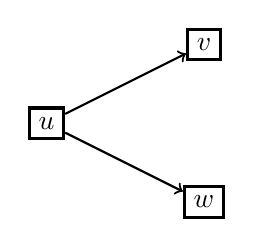
\begin{tikzpicture}[every node/.style={circle, draw, scale=1}, scale=1.0, rotate = 180]

\tikzset{every node/.style={draw, scale=1, very thick}} 
\node (today) at (3.0, 3.0) {$u$};
\node (tom1) at (1.0, 2.0) {$v$};
\node (tom2) at (1.0, 4.0) {$w$};

\tikzset{every node/.style={}}; 
\tikzset{mystyle/.style={->,thick}};  
\path (today) edge [mystyle] node {} (tom1);
\path (today) edge [mystyle] node {} (tom2);
\end{tikzpicture}
\end{center}
\caption{A frame}
\end{minipage}
\begin{minipage}[b]{0.4\linewidth}
\begin{center}
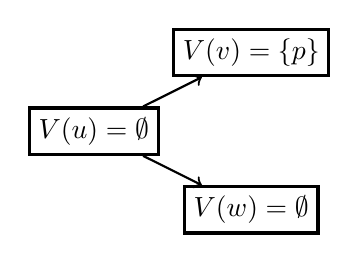
\begin{tikzpicture}[every node/.style={circle, draw, scale=1}, scale=1.0, rotate = 180]

\tikzset{every node/.style={draw, scale=1, very thick}} 
\node (today) at (3.0, 3.0) {$V(u) = \emptyset$};
\node (tom1) at (1.0, 2.0) {$V(v) = \{p\}$};
\node (tom2) at (1.0, 4.0) {$V(w) = \emptyset$};

\tikzset{every node/.style={}}; 
\tikzset{mystyle/.style={->,thick}};  
\path (today) edge [mystyle] node {} (tom1);
\path (today) edge [mystyle] node {} (tom2);
\end{tikzpicture}
\end{center}
\caption{A model}
\end{minipage}


\end{figure}

The mysterious ingredient is our \textit{Axiom K}: $\square(p \to q) \to \square p \to \square q$, or $(\square(p \to q) \wedge \square p) \to \square q$. (\textit{``If $p$ is necessarily true, and $p$ entails $q$ by necessity, then necessarily $q$ must also be true.''})

Together with (the soundness of) the Necessitation-rule (and uniform substitution), the $K$ axiom form some ``smallest'' assumptions about the behaviour of the modal connective; the \textit{normal modal logics}.

Our claim only relied on ``normality'' (very basic assumptions). What about the modality ``It is \textit{known} that $\ldots$''? If we use the box to model this modality, the necessitation-rule is the claim that ``All tautologies are known''. Philosophers often also insist that knowledge is \textit{veridical}. We can express this as the axiom $\square p \to p$ (we call this the Truth axiom, or just $T$). Other axioms stipulated in (a na\"ive) epistemic logic are: introspection; $\square p \to \square\square p$ and negative introspection $\neg \square p\to \square \neg \square p$, usually written $\lozenge p \to \square \lozenge p$ (\textit{Frame-equivalent}).
\subsection{Syntax}
$$\phi\quad ::= \quad p ~|~ \neg \phi ~|~ \phi \vee \phi ~|~ \lozenge \phi \quad\quad\text{( + abbreviations)}$$
\subsection{Semantics}
A SL-formula is evaluated against a ``truth table''. If $\prop$ is the set of propositional symbols, a configuration/instantiation/row in a truth table is some subset of $\prop$, and all possible configurations/instatiations/the entire truth table is the powerset $\wp(\prop)$.

We are not interested in ``which row is the right one'', we're interested in the \textit{validities}. Now, suppose we want to model the fact that it is not raining now, but it might (or might not) rain tomorrow. A \textit{state} is a day. 

\begin{figure}[ht]
\centering
\begin{tabular}{l|l}
\multicolumn{1}{c}{$\phi_F$ is} & \multicolumn{1}{|c}{$\phi_M$ is} \\ \hline
% & \textit{valid on the class of frames} $\mathsf F$ iff for all $\mathcal F \in \mathsf F$, $\mathcal F \Vdash \phi_M$ \\
\textit{valid} iff for all $M~:~M \vDash \phi_F$ & \textit{valid on a frame} $\mathcal F$ iff for all  $w \in \mathcal F$, $\mathcal F,w \Vdash \phi_M$\\
\textit{satisfied} in $M$ iff for all $v~:~M \vDash_v \phi_F$ & \textit{valid in a model } $M$ iff for every state $w$, $M, w \Vdash \phi_M$\\
\textit{true} w.r.t. $M$ and $v$ iff for $[\![\phi_F]\!]^M_v = 1$ & \textit{true}\footnote{Not very usual notation. Wrote it for comparison.} in $M$ at $w$ iff $w \in [\![\phi_M]\!]^M$\\
\end{tabular}
\end{figure}

Satisfaction of a formula $\phi$ in model $M = (W, R, V)$ at state $w$ is defined inductively: 
\begin{center}
\begin{tabular} {llcll}
$M, w \Vdash p $&$\iff~ p \in V(w)$ & \phantom{space} & $M, w \Vdash \phi \wedge \psi $&$\iff~ M, w \Vdash \phi \text{ and } M, w \Vdash \psi$ \\
$M, w \Vdash \neg \phi $&$\iff~ M, w \nVdash \phi$ & & $M, w \Vdash \lozenge \phi $&$\iff~ \textit{there is a }w'\in W \text{ s.t. } wRw' \text{ and } M, w' \Vdash \phi$\\
\end{tabular}
\end{center}

A Kripke model is a graph where each node is a ``SL model''. $M = (W, R, V)$ where $\bullet$ $W$ is a non-empty set of states, $\bullet R \subseteq W^2$ and $\bullet V : W \to 2^{\mathcal P}$ (coloring). A \textit{frame} is just the graph. We're usually not interested in \textit{all} graphs, but only those that satisfy certain conditions/axioms. 

\begin{proposition}Every frame satisfies the \textit{K} axiom ($\mathcal F \Vdash K$.)
\end{proposition}

\begin{proof} Let $\mathcal F$ be an arbitrary frame. Let $w$ be an arbitrary point in $\mathcal F$. Let $V$ be an arbitrary valuation over $\mathcal F$ such that $\mathcal F, V, w \Vdash \square(p \to q)$ and $\ff, V, w \Vdash \square p$ (otherwise we're done). Suppose $w$ has a neighbour $w'$ (otherwise we're done). Every $w'$ s.t. $wRw'$ satisfies $p \to q$ and $p$. It follows by MP that also every neighbour $w'$ satisfies $q$. Hence $\ff, V, w \Vdash \square q$.
\end{proof}

Certain logical axioms characterize classes of frames with certain properties. For example, the class of frames which satisfies the $T$ axiom are exactly the reflexive frames.

\begin{proposition} $\ff \Vdash T \iff Refl(\ff)$ ($T =\square p \to p \equiv^{\mathcal F} p \to \lozenge p$). \textcolor{magenta}{(Not for models; e.g., $\{p\} \to \{p\}\circlearrowleft$)}
\end{proposition}

\begin{proof} Two directions:  
\begin{description}
\item[$\Rightarrow$)] Suppose $\ff \Vdash \square p \to p$. Let $w$ be an arbitrary point and $V$ be a valuation over $\ff$ s.t. $V(w') = \{p\} \iff wRw'$. Clearly $\ff,V,w \Vdash \square p$. Since $\ff \Vdash \square p \to p$ we have, in particular $\ff, V, w\Vdash \square p \to p$ and hence, by MP, $\ff, V, w \vDash p$. By def. of $V$ we get $wRw$.
\item[$\Leftarrow)$] Notice: $\square p \to p$ and $p \to \lozenge p$ are \textit{frame equivalent}. Suppose $\ff$ is reflexive. Let $w$ be an arbitrary point in $\ff$. Let $V$ any valuation. (If $\ff, V, w \nVdash p$, we're done.) Suppose $\ff, V, w \Vdash p$, then there is a neighbour, $w$ itself, which satisfies $p$, hence $\ff, V, w \Vdash \lozenge p$.
\end{description}
\end{proof}

Similar proofs gives us $4: \square p \to \square\square p \sim$transitive, $5:\lozenge p \to \square \lozenge p\sim$Euclidean, $B: p \to \square \lozenge p \sim$symmetric, etc...

\subsection{Equivalence/Similarity}
Equivalence is defined straightforwardly:
\begin{definition}Let $\mm, \mm'$ be models and $w,w'$ be states in them.
\begin{align*}
(\mm,w) \leftrightsquigarrow (\mm',w') &\iff \{\phi ~|~ \mm, w \Vdash \phi\} = \{\phi ~|~ \mm', w' \Vdash \phi\} \\
\mm \leftrightsquigarrow \mm' &\iff \{\phi ~|~ \mm \Vdash \phi\} = \{\phi ~|~ \mm' \Vdash \phi\}\\
\end{align*}
\end{definition}

\begin{proposition} Satisfaction is invariant under generated submodels. 
\end{proposition}

\begin{proof}Let $\mm'$ be a generated submodel of $\mm$ ($\mm' \rightarrowtail \mm$), i.e., $\mm' = (W', R', V') \subseteq \mm = (W, R, V)$ s.t. 
$$V' = V|_{W'}\text{, }R' = R\cap W'^2 \text{ and for all } w \in W' ~:~ wRw'\Rightarrow  w'\in W'$$
Need to show that $w \in W'$, $\mm, w \Vdash \phi \iff \mm', w \Vdash \phi$. Structural induction on $\phi$: 
\begin{description}
\item[Base case ($p$)] Trivial.
\item[Induction step (show only $\lozenge \phi$)] Suppose $\mm, w \Vdash \lozenge \phi$. Let $w'$ be the state s.t. $wRw'$ and $\mm,w' \Vdash \phi$. By the IH we have $\mm',w'\Vdash \phi$. Since $w,w' \in W'$, $R' = R\cap W'^2$, and $(w,w') \in R$ we have $(w,w') \in R'$ and hence $\mm', w\Vdash \lozenge\phi$.\\
Suppose $\mm', w\Vdash \lozenge\phi$, then there is a state $w'$ s.t. $(w,w') \in R'$ ($\subseteq R \Rightarrow (w,w') \in R$) and $\mm', w' \Vdash \phi$. By IH we have $\mm, w'\Vdash \phi$ and the claim follows.
\end{description}
\end{proof}

Equivalence is not as fine-grained as we would like, however. 

\begin{figure}[ht]
\centering
\begin{minipage}[b]{0.35\linewidth}
\begin{center}
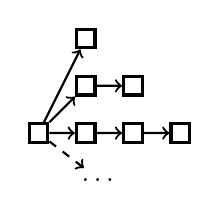
\begin{tikzpicture}[every node/.style={circle, draw, scale=1}, scale=0.6, rotate = 180]

\tikzset{every node/.style={draw, scale=1, very thick}} 
\node (11) at (3.0, 5.0) {};
\node (12) at (2.0, 3.0) {};
\node (21) at (2.0, 4.0) {};
\node (22) at (1.0, 4.0) {};
\node (31) at (2.0, 5.0) {};
\node (32) at (1.0, 5.0) {};
\node (33) at (0.0, 5.0) {};
\tikzset{every node/.style={scale=1, very thick}} 
\node (ddd) at (1.7, 6.0) {$\dots$};

\tikzset{every node/.style={}}; 
\tikzset{mystyle/.style={->,thick}};  
\path (11) edge [mystyle] node {} (12);
\path (11) edge [mystyle] node {} (21);
\path (21) edge [mystyle] node {} (22);
\path (11) edge [mystyle] node {} (31);
\path (31) edge [mystyle] node {} (32);
\path (32) edge [mystyle] node {} (33);
\tikzset{mystyle/.style={->,thick,dashed}};  
\path (11) edge [mystyle] node {} (ddd);
\end{tikzpicture}
\end{center}
\end{minipage}
\begin{minipage}[b]{0.35\linewidth}
\begin{center}
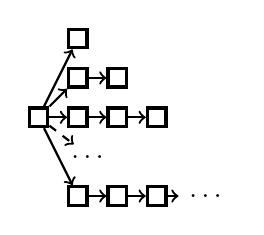
\begin{tikzpicture}[every node/.style={circle, draw, scale=1}, scale=0.5, rotate = 180]

\tikzset{every node/.style={draw, scale=1, very thick}} 
\node (11) at (3.0, 5.0) {};
\node (12) at (2.0, 3.0) {};
\node (21) at (2.0, 4.0) {};
\node (22) at (1.0, 4.0) {};
\node (31) at (2.0, 5.0) {};
\node (32) at (1.0, 5.0) {};
\node (33) at (0.0, 5.0) {};
\node (inf1) at (2.0, 7.0) {};
\node (inf2) at (1.0, 7.0) {};
\node (inf3) at (0.0, 7.0) {};
\tikzset{every node/.style={scale=1, very thick}} 
\node (infddd) at (-1.3, 7.0) {$\dots$};
\node (ddd) at (1.7, 6.0) {$\dots$};

\tikzset{every node/.style={}}; 
\tikzset{mystyle/.style={->,thick}};  
\path (11) edge [mystyle] node {} (12);
\path (11) edge [mystyle] node {} (21);
\path (21) edge [mystyle] node {} (22);
\path (11) edge [mystyle] node {} (31);
\path (31) edge [mystyle] node {} (32);
\path (32) edge [mystyle] node {} (33);
\path (11) edge [mystyle] node {} (inf1);
\path (inf1) edge [mystyle] node {} (inf2);
\path (inf2) edge [mystyle] node {} (inf3);
\path (inf3) edge [mystyle] node {} (infddd);

\tikzset{mystyle/.style={->,thick,dashed}};  
\path (11) edge [mystyle] node {} (ddd);
\end{tikzpicture}
\end{center}
\end{minipage}
\caption{Equivalent, but not bisimilar}
\end{figure}

We have natural notions of relations between (Kripke) structures. 
\begin{definition}\textbf{(Homomorphisms)} Let $M = (W, R, V), M' = (W', R', V')$ be models. A \textit{homomorphism}, denoted $f:M \to M'$, is a map $f:W \to W'$ s.t.
\begin{itemize}
\item for each $p$ and each $w \in W$, if $w \in V(p)$ then $f(w) \in V'(p)$ [[or $V(w) \subseteq V'(f(w))$]]
\item if $wRv$, then $f(w)R'f(v)$.
\end{itemize}
(A homomorphism $f : \ff \to \ff'$ for \textit{frames} from $\ff = (W, R)$ to $\ff' = (W',R')$ is a map $f:W \to W'$ s.t. $wRv~\Rightarrow~f(w)R'f(v)$.)
\end{definition}

Homomorphisms are a natural notion for relations between structures, but it doesn't yield any invariance w.r.t. satisfaction of (modal) logical formulas. \textcolor{magenta}{(A neighbourless point satisfies $\square \bot$, there is a homomorphism into a reflexive point which doesn't.)}

We could strengthen the requirement:
\begin{definition}\textbf{(Strong homomorphism)} As above, but:
\begin{itemize}
\item $w \in V(p) \iff f(w) \in V'(p)$ [[or $V(w) = V'(f(w))$]]
\item $wRv$ \textit{iff} $f(w)R'f(v)$
\end{itemize}
\end{definition}

This gives some invariance results (e.g., $\bullet$ surjective strong homom. $f : M \to M'$, then $w \meq f(w)$, $\bullet$ $M \iso M' \Rightarrow M \meq M'$.), 
but many morphisms which give invariance fail to be strong homomorphisms \textcolor{magenta}{(e.g., $f : \{u \to v \circlearrowleft\} \to \{w\circlearrowleft\}$)}. Isomorphisms are bijective strong homomorphisms.

\begin{definition}\textbf{(Bounded Morphisms)} Let $f: M = (W, R, V) \to M' = (W', R', V')$ be a homomorphism s.t.
\begin{itemize}
\item $p \in V(w)$ \textit{iff} $p \in V'(f(w))$
\item \textit{moot bc homom.:} $wRv$ then $f(w)Rf(v)$, and
\item $f(w)R'v' \Rightarrow$ $wRv$ for some $v$ s.t. $f(v) = v'$ (the \textit{Back} condition).
\end{itemize}
\end{definition}

\begin{figure}[ht]
\begin{minipage}[b]{0.4\linewidth}
\begin{center}
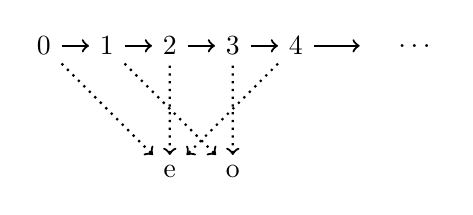
\begin{tikzpicture}[every node/.style={circle, draw, scale=1}, scale=0.8, rotate = 180]
\tikzset{every node/.style={scale=1, very thick}} 
\node (n0) at (5.0, 0.0) {0};
\node (n1) at (4.0, 0.0) {1};
\node (n2) at (3.0, 0.0) {2};
\node (n3) at (2.0, 0.0) {3};
\node (n4) at (1.0, 0.0) {4};
\node (ddd) at (-0.7, 0.0) {$\quad\dots$};
\node (e) at (3.0, 2.0) {e};
\node (o) at (2.0, 2.0) {o};

\tikzset{every node/.style={}}; 
\tikzset{mystyle/.style={->,thick}};  
\path (n0) edge [mystyle] node {} (n1);
\path (n1) edge [mystyle] node {} (n2);
\path (n2) edge [mystyle] node {} (n3);
\path (n3) edge [mystyle] node {} (n4);
\path (n4) edge [mystyle] node {} (ddd);

\tikzset{mystyle/.style={->,thick,dotted}};  
\path (n0) edge [mystyle] node {} (e);
\path (n1) edge [mystyle] node {} (o);
\path (n2) edge [mystyle] node {} (e);
\path (n3) edge [mystyle] node {} (o);
\path (n4) edge [mystyle] node {} (e);
\end{tikzpicture}
\end{center}
\caption{Bounded, not strong (one way!)}
\end{minipage}
\begin{minipage}[b]{0.4\linewidth}
\begin{center}
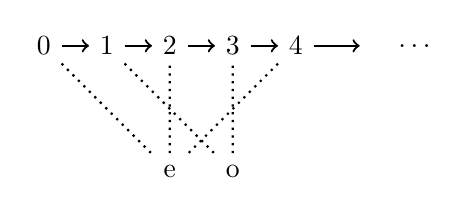
\begin{tikzpicture}[every node/.style={circle, draw, scale=1}, scale=0.8, rotate = 180]
\tikzset{every node/.style={scale=1, very thick}} 
\node (n0) at (5.0, 0.0) {0};
\node (n1) at (4.0, 0.0) {1};
\node (n2) at (3.0, 0.0) {2};
\node (n3) at (2.0, 0.0) {3};
\node (n4) at (1.0, 0.0) {4};
\node (ddd) at (-0.7, 0.0) {$\quad\dots$};
\node (e) at (3.0, 2.0) {e};
\node (o) at (2.0, 2.0) {o};

\tikzset{every node/.style={}}; 
\tikzset{mystyle/.style={->,thick}};  
\path (n0) edge [mystyle] node {} (n1);
\path (n1) edge [mystyle] node {} (n2);
\path (n2) edge [mystyle] node {} (n3);
\path (n3) edge [mystyle] node {} (n4);
\path (n4) edge [mystyle] node {} (ddd);

\tikzset{mystyle/.style={-,thick,dotted}};  
\path (n0) edge [mystyle] node {} (e);
\path (n1) edge [mystyle] node {} (o);
\path (n2) edge [mystyle] node {} (e);
\path (n3) edge [mystyle] node {} (o);
\path (n4) edge [mystyle] node {} (e);
\end{tikzpicture}
\end{center}
\caption{Bisimilar (coming up)}
\end{minipage}
\end{figure}


\subsection{Bisimulation}
\begin{definition} If $M = (W, R, V)$ and $M' = (W', R', V')$ are models and $Z \subseteq W \times W'$, then $M \bisim M'$ \textit{iff}
\begin{description}
\item[Propositional agreement] if $wZw'$, then $V(w) = V'(w')$, 
\item[Forth] If $wZw'$ and $wRv$, then there is a $v'$ s.t. $vZv'$ and $w'R'v'$, and
\item[Back] If $wZw'$ and $w'R'v'$, then there is a $v$ s.t. $vZv'$ and $wRv$.
\end{description}
\end{definition}

\begin{figure}[ht]
\begin{minipage}[b]{0.3\linewidth}
\begin{center}
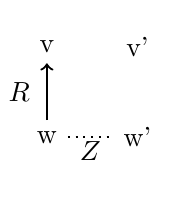
\begin{tikzpicture}[every node/.style={circle, draw, scale=1}, scale=0.23, rotate = 180]
\tikzset{every node/.style={scale=1, very thick}} 
\node (w) at (5.0, 5.0) {w};
\node (v) at (5.0, 0.0) {v};
\node (ww) at (0.0, 5.0) {w'};
\node (vv) at (0.0, 0.0) {v'};
\tikzset{every node/.style={scale=1, very thick}} 

\tikzset{every node/.style={}}; 
\tikzset{mystyle/.style={->,thick}};  
\path (w) edge [mystyle] node {$\hspace{-2em}R$} (v);
\tikzset{mystyle/.style={-,thick,dotted}};  
\path (w) edge [mystyle] node {$\begin{matrix} \\ Z \end{matrix}$} (ww);

\tikzset{mystyle/.style={->,thick,dashed}};  
\end{tikzpicture}
\end{center}
\end{minipage}
\begin{minipage}[b]{0.3\linewidth}
\begin{center}
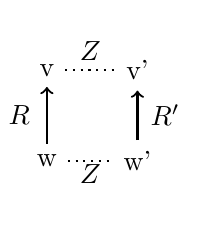
\begin{tikzpicture}[every node/.style={circle, draw, scale=1}, scale=0.23, rotate = 180]
\tikzset{every node/.style={scale=1, very thick}} 
\node (w) at (5.0, 5.0) {w};
\node (v) at (5.0, 0.0) {v};
\node (ww) at (0.0, 5.0) {w'};
\node (vv) at (0.0, 0.0) {v'};
\tikzset{every node/.style={scale=1, very thick}} 

\tikzset{every node/.style={}}; 
\tikzset{mystyle/.style={->,thick}};  
\path (w) edge [mystyle] node {$\hspace{-2em}R$} (v);
\path (ww) edge [mystyle] node {$\hspace{2em}R'$} (vv);
\tikzset{mystyle/.style={-,thick,dotted}};  
\path (w) edge [mystyle] node {$\begin{matrix} \\ Z \end{matrix}$} (ww);
\path (v) edge [mystyle] node {$\begin{matrix} Z \\ \phantom{Haxord!}\end{matrix}$} (vv);

\tikzset{mystyle/.style={->,thick,dashed}};  
\end{tikzpicture}
\end{center}
\end{minipage}
\begin{minipage}[b]{0.3\linewidth}
\begin{center}
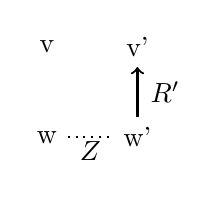
\begin{tikzpicture}[every node/.style={circle, draw, scale=1}, scale=0.23, rotate = 180]
\tikzset{every node/.style={scale=1, very thick}} 
\node (w) at (5.0, 5.0) {w};
\node (v) at (5.0, 0.0) {v};
\node (ww) at (0.0, 5.0) {w'};
\node (vv) at (0.0, 0.0) {v'};
\tikzset{every node/.style={scale=1, very thick}} 

\tikzset{every node/.style={}}; 
\tikzset{mystyle/.style={->,thick}};  
\path (ww) edge [mystyle] node {$\hspace{2em}R'$} (vv);
\tikzset{mystyle/.style={-,thick,dotted}};  
\path (w) edge [mystyle] node {$\begin{matrix} \\ Z \end{matrix}$} (ww);

\tikzset{mystyle/.style={->,thick,dashed}};  
\end{tikzpicture}
\end{center}
\end{minipage}
%\caption*{Forth $\Longrightarrow\hspace{14em}\Longleftarrow$ Back}
\end{figure}

\begin{proposition}Modal formulas are invariant under bisimulation ($w \bisim w' \Rightarrow w \leftrightsquigarrow w'$).
\label{prop:bisim-imp-eq}
\end{proposition}

\begin{proof}Let $M,w$ and $M',w'$ be pointed models such that $w \bisim w'$. Induction on $\phi$. 
\begin{description}
\item[Base case ($p$)] By def.
\item[Induction step: ($\lozenge \phi$)] Suppose $M, w \Vdash \lozenge \phi$, then $wRv$ and $M, v \Vdash \phi$. But since $w\bisim w'$, there is a $v'$ s.t. $w'R'v'$ and $v \bisim v'$. By IH it follows that $M', v' \Vdash \phi$, and hence $M', w \Vdash \lozenge\phi$.
\end{description}
\end{proof}
When is the converse true? 
\begin{proposition} (\textbf{Hennessy-Milner Theorem}) Let $M = (W, R, V)$ and $M' = (W', R', V')$ be two \textit{image-finite} models (every $w$, $|R_{trg}(w)| \in \mathbb N$). For every $w \in W$ and $w' \in W'$, $w \bisim w' \iff w \leftrightsquigarrow w'$. 
\end{proposition}

\begin{proof}
$\Rightarrow$) is done (Prop. \ref{prop:bisim-imp-eq}). $\Leftarrow$) Prove that $\leftrightsquigarrow$ is a bisimulation relation on these models.

$\leftrightsquigarrow$ clearly satisfies \textbf{Propositional Agreement}. Now, for \textbf{Forth}, suppose $w \leftrightsquigarrow w'$ and $wRv$. Suppose towards a contradiction that there is no $v'$ in $M'$ such that $w'R'v'$ and $v \meq v'$. Notice:
\begin{itemize}
\item $M, w \Vdash \lozenge \top$ (has a successor), and since $w \meq w'$, 
\item $R_{trg}(w')$ is non-empty and finite (from \textit{image-finite}).
\end{itemize}
Let's say $R_{trg}(w') = \{w_1', w_2', \dots, w_n'\}$. By assumption (no $v' \in R_{trg}(w') \meq v \in R_{trg}(w)$), there is a formula for each $w_i'$, say $\psi_i$ s.t. $M, v \Vdash \psi_i$, but $M', w_i' \Vdash \psi_i$ (otherwise they would be equivalent!). But then 
$$M, w \Vdash \lozenge (\psi_1 \wedge \dots \wedge \psi_n) \text{ and } M', w' \nVdash \lozenge(\psi_1 \wedge \ldots \wedge \psi_n)$$
which contradicts our assumption that $w \meq w'$. \textcolor{magenta}{Using the fact that formulas are finite.}
\end{proof}

Bisimulation is cool because:\begin{enumerate}
\item It's behavioural/observational like we want when talking about LTSs.
\item It's is a more fine-grained measure of similarity than equivalence, but not so fine-grained that it distinguishes modally indistinguishable models.
\item ``The quotient of a model w.r.t. its largest auto-bisimulation can be regarded as a minimal representation of this model.'' [BB]
\item Two non-wellfounded sets are considered equal if their decoration graphs are bisimilar. [$\sim$BB]
\item Modal logic is \textit{the} fragment of FOL which is closed under bisimulation (van Benthem Characterization Theorem).
\end{enumerate}

\subsection{Frames as coalgebras}
A frame is a graph $(W, R)$. The relation $R$ can be represented as a map $W \to \wp(W)$, i.e., a morphism in $\mathsf{Set}$. And waddayano, it fits our coalg(functor)-picture. 

\begin{figure}[ht]
\begin{minipage}[b]{0.5\linewidth}
\begin{center}
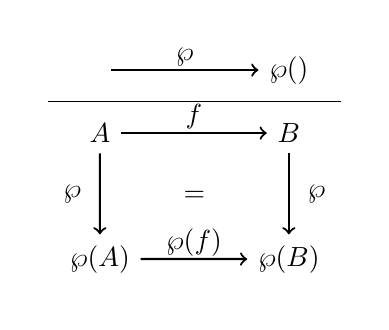
\begin{tikzpicture}[every node/.style={circle, draw, scale=1}, scale=0.8, rotate = 180]

\tikzset{every node/.style={scale=1, very thick}} 
\node (x) at (3.0, 0.0) {$\xx$};
\node (sx) at (0.0, 0.0) {$\wp(\xx)$};

\node (e0) at (4.0, 0.5) {};
\node (e1) at (-1.0, 0.5) {};
\node (eq) at (1.5, 2.0) {$=$};

\node (A) at (3.0, 1.0) {$A$};
\node (B) at (0.0, 1.0) {$B$};
\node (pA) at (3.0, 3.0) {$\wp(A)$};
\node (pB) at (0.0, 3.0) {$\wp(B)$};

\tikzset{every node/.style={}}; 
\tikzset{mystyle/.style={-,thin}};  
\path (e0) edge [mystyle] node {} (e1);
\tikzset{mystyle/.style={->,thick}};  
\path (x) edge [mystyle] node {$\begin{matrix} \wp \\ \\ \end{matrix}$} (sx);

\tikzset{mystyle/.style={->,thick}};  
\path (A) edge [mystyle] node {$\begin{matrix} f \\ \\ \end{matrix}$} (B);
\path (pA) edge [mystyle] node {$\begin{matrix} \wp(f) \\ \\ \end{matrix}$} (pB);
\path (A) edge [mystyle] node {$\wp\hspace{2em}$} (pA);
\path (B) edge [mystyle] node {$\hspace{2em}\wp$} (pB);

\end{tikzpicture}
\end{center}
\caption{$\wp$ is an endo-functor on $\mathsf{Set}$}
\label{fig:frame-in-set}
\end{minipage}
\begin{minipage}[b]{0.45\linewidth}
\begin{center}
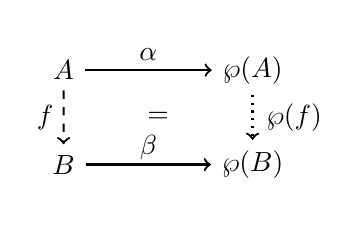
\begin{tikzpicture}[every node/.style={circle, draw, scale=1}, scale=0.8, rotate = 180]
\tikzset{every node/.style={scale=1, very thick}} 
\node (A) at (3.0, 0.0) {$A$};
\node (sA) at (0.0, 0.0) {$\wp(A)$};
\node (B) at (3.0, 1.5) {$B$};
\node (sB) at (0.0, 1.5) {$\wp(B)$};

\node (commute) at (1.5, 0.75) {$=$};

\tikzset{every node/.style={}}; 
\tikzset{mystyle/.style={->,thick}};  
\path (A) edge [mystyle] node {$\begin{matrix} \alpha \\ \\ \end{matrix}$} (sA);
\path (B) edge [mystyle] node {$\begin{matrix} \beta \\ \\ \end{matrix}$} (sB);
\tikzset{mystyle/.style={->,thick,dashed}};  
\path (A) edge [mystyle] node {$f~\quad$} (B);
\tikzset{mystyle/.style={->,thick,dotted}};  
\path (sA) edge [mystyle] node {$\hspace{3em} \wp(f)$} (sB);

\end{tikzpicture}
\end{center}
\caption{Frames as $(A,\alpha)$ (coalg) in $\mathsf{Set}$}
\label{fig:morphism-in-frame}
\end{minipage}
\end{figure}

\begin{figure}[ht]
\begin{center}
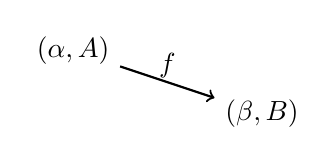
\begin{tikzpicture}[every node/.style={circle, draw, scale=1}, scale=0.8, rotate = 180]

\tikzset{every node/.style={scale=1, very thick}} 
\node (x) at (3.0, 0.0) {$(\alpha,A)$};
\node (sx) at (0.0, 1.0) {$(\beta, B)$};

\tikzset{every node/.style={}}; 
\tikzset{mystyle/.style={->,thick}};  
\path (x) edge [mystyle] node {$\begin{matrix} f \\ \\ \end{matrix}$} (sx);
\end{tikzpicture}
\end{center}
\caption{Frames as obj in $\mathsf{Coalg}(\wp)$}
\label{fig:frame-coalg}
\end{figure}

A functor is a map $F : \mathbb C \to \mathbb D$ such that $\bullet$ for any object $c$ in $\mathbb C$, $F(c)$ is an object in $\mathbb D$, $\bullet$ when $f : c \to c'$ is a morphism in $\mathbb C$, then $F(f) : F(c) \to F(c')$ is a morphism in $\mathbb D$, $\bullet~$ $F(Id_c) = Id_{F(c)}$, and $\bullet ~ F(f;g) = F(f);F(g)$.

\begin{proposition}\textbf{Figure \ref{fig:frame-in-set}} is an (endo-)functor in $\mathsf{Set}$ .\end{proposition}

\begin{proof} Let $f : A \to B$. $\wp(f)(S) = \{f(x) ~|~ x \in S\}$. 

$F(f;g)(S) = \{ (f;g)(x) ~|~ x \in S\} = \{ g(y) ~|~ y = f(x), x \in S\} =  \{g (y) ~|~ y \in \{ f(x) ~|~ x \in S\}\} = \{g (y) ~|~ y \in F(f)(S)\} $\\
$= (F(f);F(g))(S)$
\end{proof}

\textbf{Figure \ref{fig:morphism-in-frame}} is just like half of Figure \ref{fig:frame-in-set}, but nicer, rotated, and a bit squashed.

\begin{definition}
Morphisms in $\mathsf{Coalg}(\wp)$ ($f : (\alpha, A) \to (\beta, B)$ in \textbf{Figure \ref{fig:frame-coalg}}) are maps $f : A \to B$ such that 
\begin{enumerate}
\item $y \in \alpha(x) ~\Rightarrow~ f(y) \in \beta(f(x))$ [[or $x(\alpha)y ~\Rightarrow~ f(x)(\beta)f(y)$, or $xRy ~\Rightarrow~ f(x)R'f(y)$]]
\item $y' \in \beta(f(x)) \Rightarrow \exists y$ s.t. $y \in \alpha(x)$ and $f(y) = y'$.
\end{enumerate}
\end{definition}
\begin{figure}[ht]
\centering
\begin{minipage}[b]{0.5\linewidth}
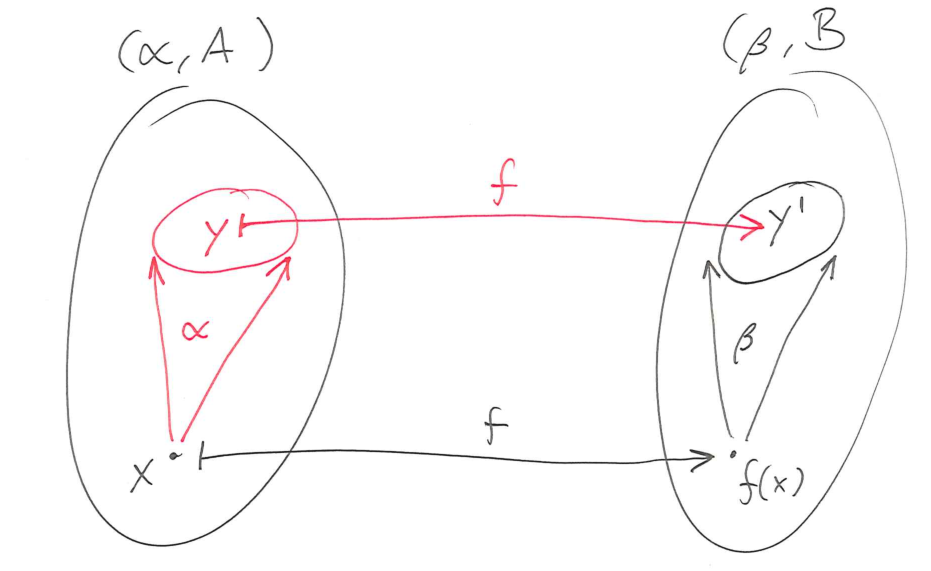
\includegraphics[scale=0.4]{frame-coalg-morphism-2.pdf}
\end{minipage}
\begin{minipage}[b]{0.4\linewidth}
That is to say:
\begin{enumerate}
\item $f_{\wp}(\alpha(x)) \subseteq \beta(f(x))$, and
\item $\beta(f(x)) \subseteq f_\wp(\alpha(x))$
\end{enumerate}

Or just 
$$\alpha;f_\wp = f;\beta$$
$\vspace{3em}$
\end{minipage}
\caption{(2) says ``If $f:(\alpha, A) \to (\beta, B)$ and we've got the black, we also have the red''.}
\end{figure}



\subsection{Models as coalgebras}
Models have type-functor $F : \xx \to \wp(\prop) \times \wp(\xx)$. Since we don't care about all the propositional symbols we can simplify to $F : \xx \to C \times \wp(\xx)$. We can think of an element in $C$ as a row in a truthtable or a color or whatever.

\begin{figure}[ht]
\centering
\begin{minipage}[b]{0.4\linewidth}
\begin{center}
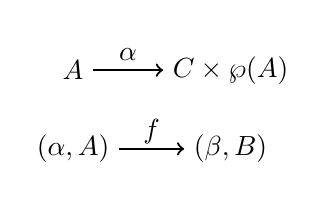
\begin{tikzpicture}
\node (A) at (0.0, 1.0) {$A$};
\node (trg) at (2.0, 1.0) {$C\times\wp(A)$};
\node (aA) at (0.0, 0.0) {$(\alpha, A)$};
\node (bB) at (2.0, 0.0) {$(\beta, B)$};

\tikzset{mystyle/.style={->,thick}};  
\path (A) edge [mystyle] node {$\begin{matrix}\alpha \\~ \end{matrix}$} (trg);
\path (aA) edge [mystyle] node {$\begin{matrix}f \\ ~\end{matrix}$} (bB);
\end{tikzpicture}
\end{center}
\caption{Model \& Morphism}
\label{fig:coalg-mod-and-morph}
\end{minipage}
\begin{minipage}[b]{0.5\linewidth}
\begin{center}
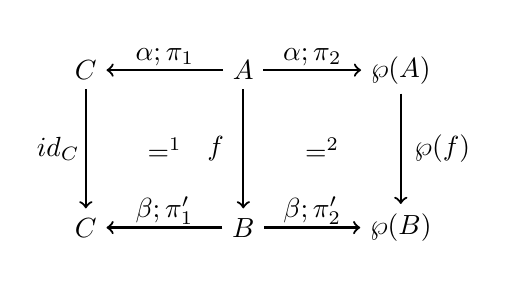
\begin{tikzpicture}
\node (A) at (0.0, 2.0) {$A$};
\node (B) at (0.0, 0.0) {$B$};

\node (CA) at (-2.0, 2.0) {$C$};
\node (sA) at (2.0, 2.0) {$\wp(A)$};

\node (CB) at (-2.0, 0.0) {$C$};
\node (sB) at (2.0, 0.0) {$\wp(B)$};

\node (eq2) at (-1.0, 1.0) {$=^1$};
\node (eq1) at (1.0, 1.0) {$=^2$};

\tikzset{mystyle/.style={->,thick}};  
\path (A) edge [mystyle] node {$f\hspace{2em}$} (B);
\path (A) edge [mystyle] node {$\begin{matrix}\alpha;\pi_1 \\ ~\end{matrix}$} (CA);
\path (A) edge [mystyle] node {$\begin{matrix}\alpha;\pi_2 \\ ~\end{matrix}$} (sA);

\path (B) edge [mystyle] node {$\begin{matrix}\beta;\pi'_1 \\ ~\end{matrix}$} (CB);
\path (B) edge [mystyle] node {$\begin{matrix}\beta;\pi'_2 \\ ~\end{matrix}$} (sB);

\path (CA) edge [mystyle] node {$id_C\hspace{2em}$} (CB);
\path (sA) edge [mystyle] node {$\hspace{3em}\wp(f)$} (sB);
\end{tikzpicture}
\end{center}
\caption{Morphism condition}
\label{fig:mod-morph-cond}
\end{minipage}
\end{figure}

\begin{figure}[ht]
\begin{center}
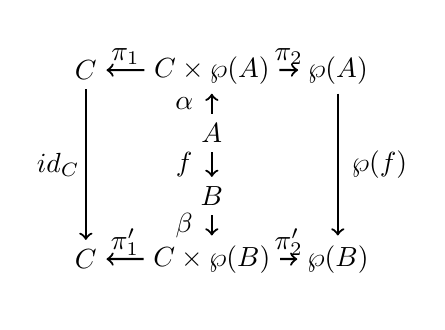
\begin{tikzpicture}[scale=0.4]
\node (A) at (0.0, 2.0) {$A$};
\node (CxpA) at (0.0, 4.0) {$C\times\wp(A)$};
\node (B) at (0.0, 0.0) {$B$};
\node (CxpB) at (0.0, -2.0) {$C \times \wp(B)$};

\node (CA) at (-4.0, 4.0) {$C$};
\node (sA) at (4.0, 4.0) {$\wp(A)$};

\node (CB) at (-4.0, -2.0) {$C$};
\node (sB) at (4.0, -2.0) {$\wp(B)$};

\tikzset{mystyle/.style={->,thick}};  
\path (A) edge [mystyle] node {$f\hspace{2em}$} (B);

\path (A) edge [mystyle] node {$\alpha\hspace{2em}$} (CxpA);
\path (B) edge [mystyle] node {$\beta\hspace{2em}$} (CxpB);

\path (CA) edge [mystyle] node {$id_C\hspace{2em}$} (CB);
\path (sA) edge [mystyle] node {$\hspace{3em}\wp(f)$} (sB);

\path (CxpA) edge [mystyle] node {$\begin{matrix}{\pi_1} \\ ~\end{matrix}$} (CA);
\path (CxpA) edge [mystyle] node {$\begin{matrix}{\pi_2} \\ ~\end{matrix}$} (sA);

\path (CxpB) edge [mystyle] node {$\begin{matrix}{\pi'_1} \\ ~\end{matrix}$} (CB);
\path (CxpB) edge [mystyle] node {$\begin{matrix}{\pi'_2} \\ ~\end{matrix}$} (sB);
\end{tikzpicture}
\end{center}
\caption{More verbose}
\end{figure}
\begin{minipage}[b]{0.6\linewidth}
A morphism in $\mathsf{Coalg}(C\times \wp)$ is a map $f : (\alpha, A) \to (\beta, B)$ (as in Figure \ref{fig:coalg-mod-and-morph}), such that the diagram in Figure \ref{fig:mod-morph-cond} commutes.

In Figure \ref{fig:mod-morph-cond} the two statements express ($=^1$): $a \in A$ and $f(a) \in B$ have the same coloring, and ($=^2$): the same as for frames (simulation).

Let's look at an example of two objects in $\mathsf{Coalg}(C\times \wp)$: 
\end{minipage}
\begin{minipage}[b]{0.3\linewidth}
\begin{center}
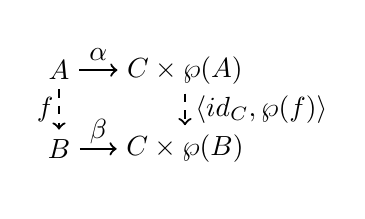
\begin{tikzpicture}
\node (A) at (0.0, 1.0) {$A$};
\node (trgA) at (1.6, 1.0) {$C\times\wp(A)$};
\node (B) at (0.0, 0.0) {$B$};
\node (trgB) at (1.6, 0.0) {$C\times\wp(B)$};

\tikzset{mystyle/.style={->,thick}};  
\path (A) edge [mystyle] node {$\begin{matrix}\alpha \\~ \end{matrix}$} (trgA);
\path (B) edge [mystyle] node {$\begin{matrix}\beta \\ ~\end{matrix}$} (trgB);
\tikzset{mystyle/.style={->,thick,dashed}};  
\path (A) edge [mystyle] node {$f\quad$} (B);
\path (trgA) edge [mystyle] node[right]{$\langle id_C, \wp(f) \rangle$} (trgB);
\end{tikzpicture}\\
\textsc{Actual Figure 13. } 
\end{center}
\end{minipage}


Let $A = \{1, 2, 3, 4, 5\}$, and $\alpha(1) = (c_1, \{2\}), \alpha(2) = (c_2, \{3\}), \alpha(3) = (c_1, \{4, 5\}) \alpha(4) = (c_2, \emptyset)$, and $\alpha(5) = (c_2, \emptyset)$.

Let $B = \{a, b, c, d, e\}$, and $\beta(a) = (c_1, \{b, c\}), \beta(b) = (c_2, \{d\}), \beta(c) = (c_2, \{d\}), \beta(d) = (c_1, \{e\})$, and $\beta(e) = (c_2, \emptyset)$.

Is there a morphism from $(\alpha, A)$ to $(\beta, B)$? Indeed there is. Let $f = \{1 \mapsto a, 2 \mapsto b, 3 \mapsto b, 4 \mapsto e, 5 \mapsto e\}$.



\subsection{Canonical models are final objects}
\truls{This subsection is controversial. Do not trust it!}
The elements in the category $\mathsf{Coalg}(\wp(P)\times\wp(A)) = \mathcal C$ are extactly all Kripke models (all models over arbitrary frames). Let $\mathfrak M^C$ be the canonical model for the the logic \textit{K}. A morphism in $\mathcal C$ is a bounded morphism from one model to another (as sketched above), i.e., a map from states to states such that (...)

\begin{proposition}
The unique bounded morphism $id_{\mathfrak M^C} : \mathfrak M^C \to \mathfrak M^C$ is the identity map (mapping each state (maximal consistent set of formulas) to itself).\end{proposition}


\begin{proof} Two claims:
\begin{description}
\item[Bounded morphism] the identity map $id_{\mathfrak M^C}$ is a bounded morphism.
\item[Unique] Suppose there was a bounded morphism $f : \mathfrak M^C \to \mathfrak M^C$ distinct from the identity map. Then there is some state $w$ such that $w \neq f(w)$. Let $\phi \in w$. We show that $\phi \in f(w)$. We prove the claim $\phi \in w \Leftrightarrow \phi \in f(w)$ by induction on $\phi$:
\begin{description}
\item[Base case ($p$)] $p \in w \Leftrightarrow w \Vdash p$, but since $f$ is a bounded morphism, $f(w) \Vdash p$, so $p \in f(w)$.
\item[Induction step(s)] Boolean cases are simple.
\begin{description}
\item[$\phi = \neg \psi$] $\neg \psi \in w \Leftrightarrow \psi \notin w$ (by the construction of $\mathfrak M^C$). By IH $\psi \notin f(w)$, and hence $\neg \psi \in f(w)$ (by construction).
\item[$\phi = \psi_1 \wedge \psi_2$] $\psi_1 \wedge \psi_2 \in w \Leftrightarrow \text{both } \psi_1 \in w \text{ and } \psi_2 \in w$ (corrolary from construction). IH yields $\psi_1,\psi_2 \in f(w)$ and definition of $\mathfrak M^C$ yields $\psi_1 \wedge \psi_2 \in f(w)$.
\item[$\phi = \lozenge \psi$] Let $v$ be an arbitrary state such that $wR^Cv$ and $v \Vdash \psi$. Since $f$ is a bounded morphism, $f(w)R^Cf(v)$. IH gives $f(v) \Vdash \psi$, but then $f(w)\Vdash \lozenge \psi$.
\end{description}
\end{description}
So $\phi \in w \Leftrightarrow \phi \in f(w)$ and $f$ needs to be the identity map.
\end{description}
So $id_{\mathfrak M^C}$ is the unique bounded morphism in $\mathcal C$ from $\mathfrak M^C$ to itself.
\end{proof}

A morphism from an arbitrary model into the canonical model is unique modulo the choice of how to extend a set of formulas to maximal sets.
\begin{proof} Here is a quote:
\begin{quote}
Grif: ``You can't call dibs on a spaceship! That's ridiculous!''
\begin{flushright}
from \textit{Red vs. Blue}, Season 5, Ep. \textit{``You can't park here''}
\end{flushright}
\end{quote}
\end{proof}



\end{document}

